
\chapter[Implementation]{Implementation}
\graphicspath{ {images/implementation} }
In this chapter, we present how we designed and implemented SYN, a tool that implements our approach described in the previous Chapter.

\section{Platform Overview}
SYN is our tool to visualize and auralize a system's evolution. 
It is composed of a set of modules, as follows:
\begin{itemize}
    \item \textbf{Core}: it holds classes representing basic SYN concepts such as ProjectHistories, ProjectVersions, and FileVersions. It also provides abstract classes, open to any implementation, to achieve the extensibility goal.
    \item \textbf{CLI}: provides a Command Line Interface (CLI) to users.
    \item \textbf{Analyzer}: implements the analysis approach described in \autoref{s:EvolutionModel}. 
    \item \textbf{Server}: provides GraphQL endpoints to retrieve data. 
    \item \textbf{Visual Inspector}: the user interface to debug and visually depict information collected during the analysis. 
\end{itemize}

All the modules of SYN are written in Java, except the Visual Inspector, which is written with React and TypeScript. 

A user has two options to interact with SYN: through the console with the commands provided by the CLI module 
or through a web application embedded in the Visual Inspector module.
\autoref{fig:architecture} gives a high-level overview of the architecture. Arrows represent the dependencies among the modules.
The heart of the system is the Core module. It implements the core model and provides classes to standardize the communication among the modules.
There is also a class called ViewGenerator, in the core to create views over the collected repository's data.
The Analyzer module has classes that act as a repository explorer to retrieve data from the repository history. 
Moreover, metrics are extracted with the metrics extractor component and put inside each FileVersion through the history builder component. 
CLI provides commands that directly call functions defined inside Analyzer. 
This is why it has both Core and Analyzer as dependencies. 

The Visual Inspector holds the Graphical User Interface (GUI) of SYN. Information is retrieved through endpoints specified by the GraphQL server of the Server module, which, in turn, retrieves view data from the Core module. 


\begin{figure}
    \center
    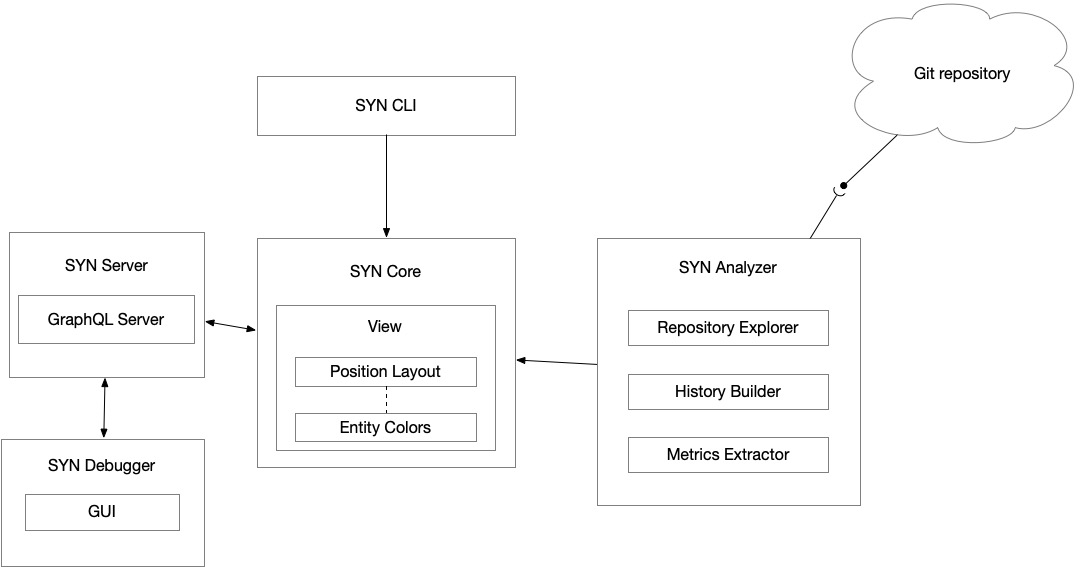
\includegraphics[width=\textwidth]{SYNArchitecture.jpg}
    \caption{Architecture of SYN}
    \label{fig:architecture}
\end{figure}

%Having reached a low coupling between modules, the extensibility of SYN is preserved.
Modules such as SYN Server or Analyzer implementation could be changed without altering the codebase of other modules. 

\section{Core}
SYN Core is the module that holds all the entities introduced in \autoref{s:EvolutionModel}. 
All the classes of our abstraction extend the \texttt{Entity} class, composed of the field \texttt{id}, to identify an object inside our domain. 
Classes inside the model of Core could be partitioned into four subdomains: Project, History, Analysis, and View. 

\subsection*{Project}
The first part of the model consists of the \textbf{Project} entities. 
The class diagram is shown in \autoref{fig:SYNCLass}. The abstract class \texttt{Project} represents a software system. It defines the following fields:
\begin{itemize}
    \item \texttt{name}
    \item \texttt{projectHistory}: an object that represents the project's history. It holds the results of the analysis. 
    \item \texttt{path}: the path of the analyzed git repository. 
\end{itemize}

We defined two additional classes: \texttt{LocalProject} to represent a project in the local storage and \texttt{RemoteProject} to describe a project that needs to be retrieved from a remote source. 
\texttt{LocalProject} does not need any further fields to represent a local project, \texttt{RemoteProject} has a \texttt{projectURL} field. We might add more information, such as the git branch or the remote credentials; despite that, we decided to keep the implementation as simple as possible. 


\begin{figure}
    \center
    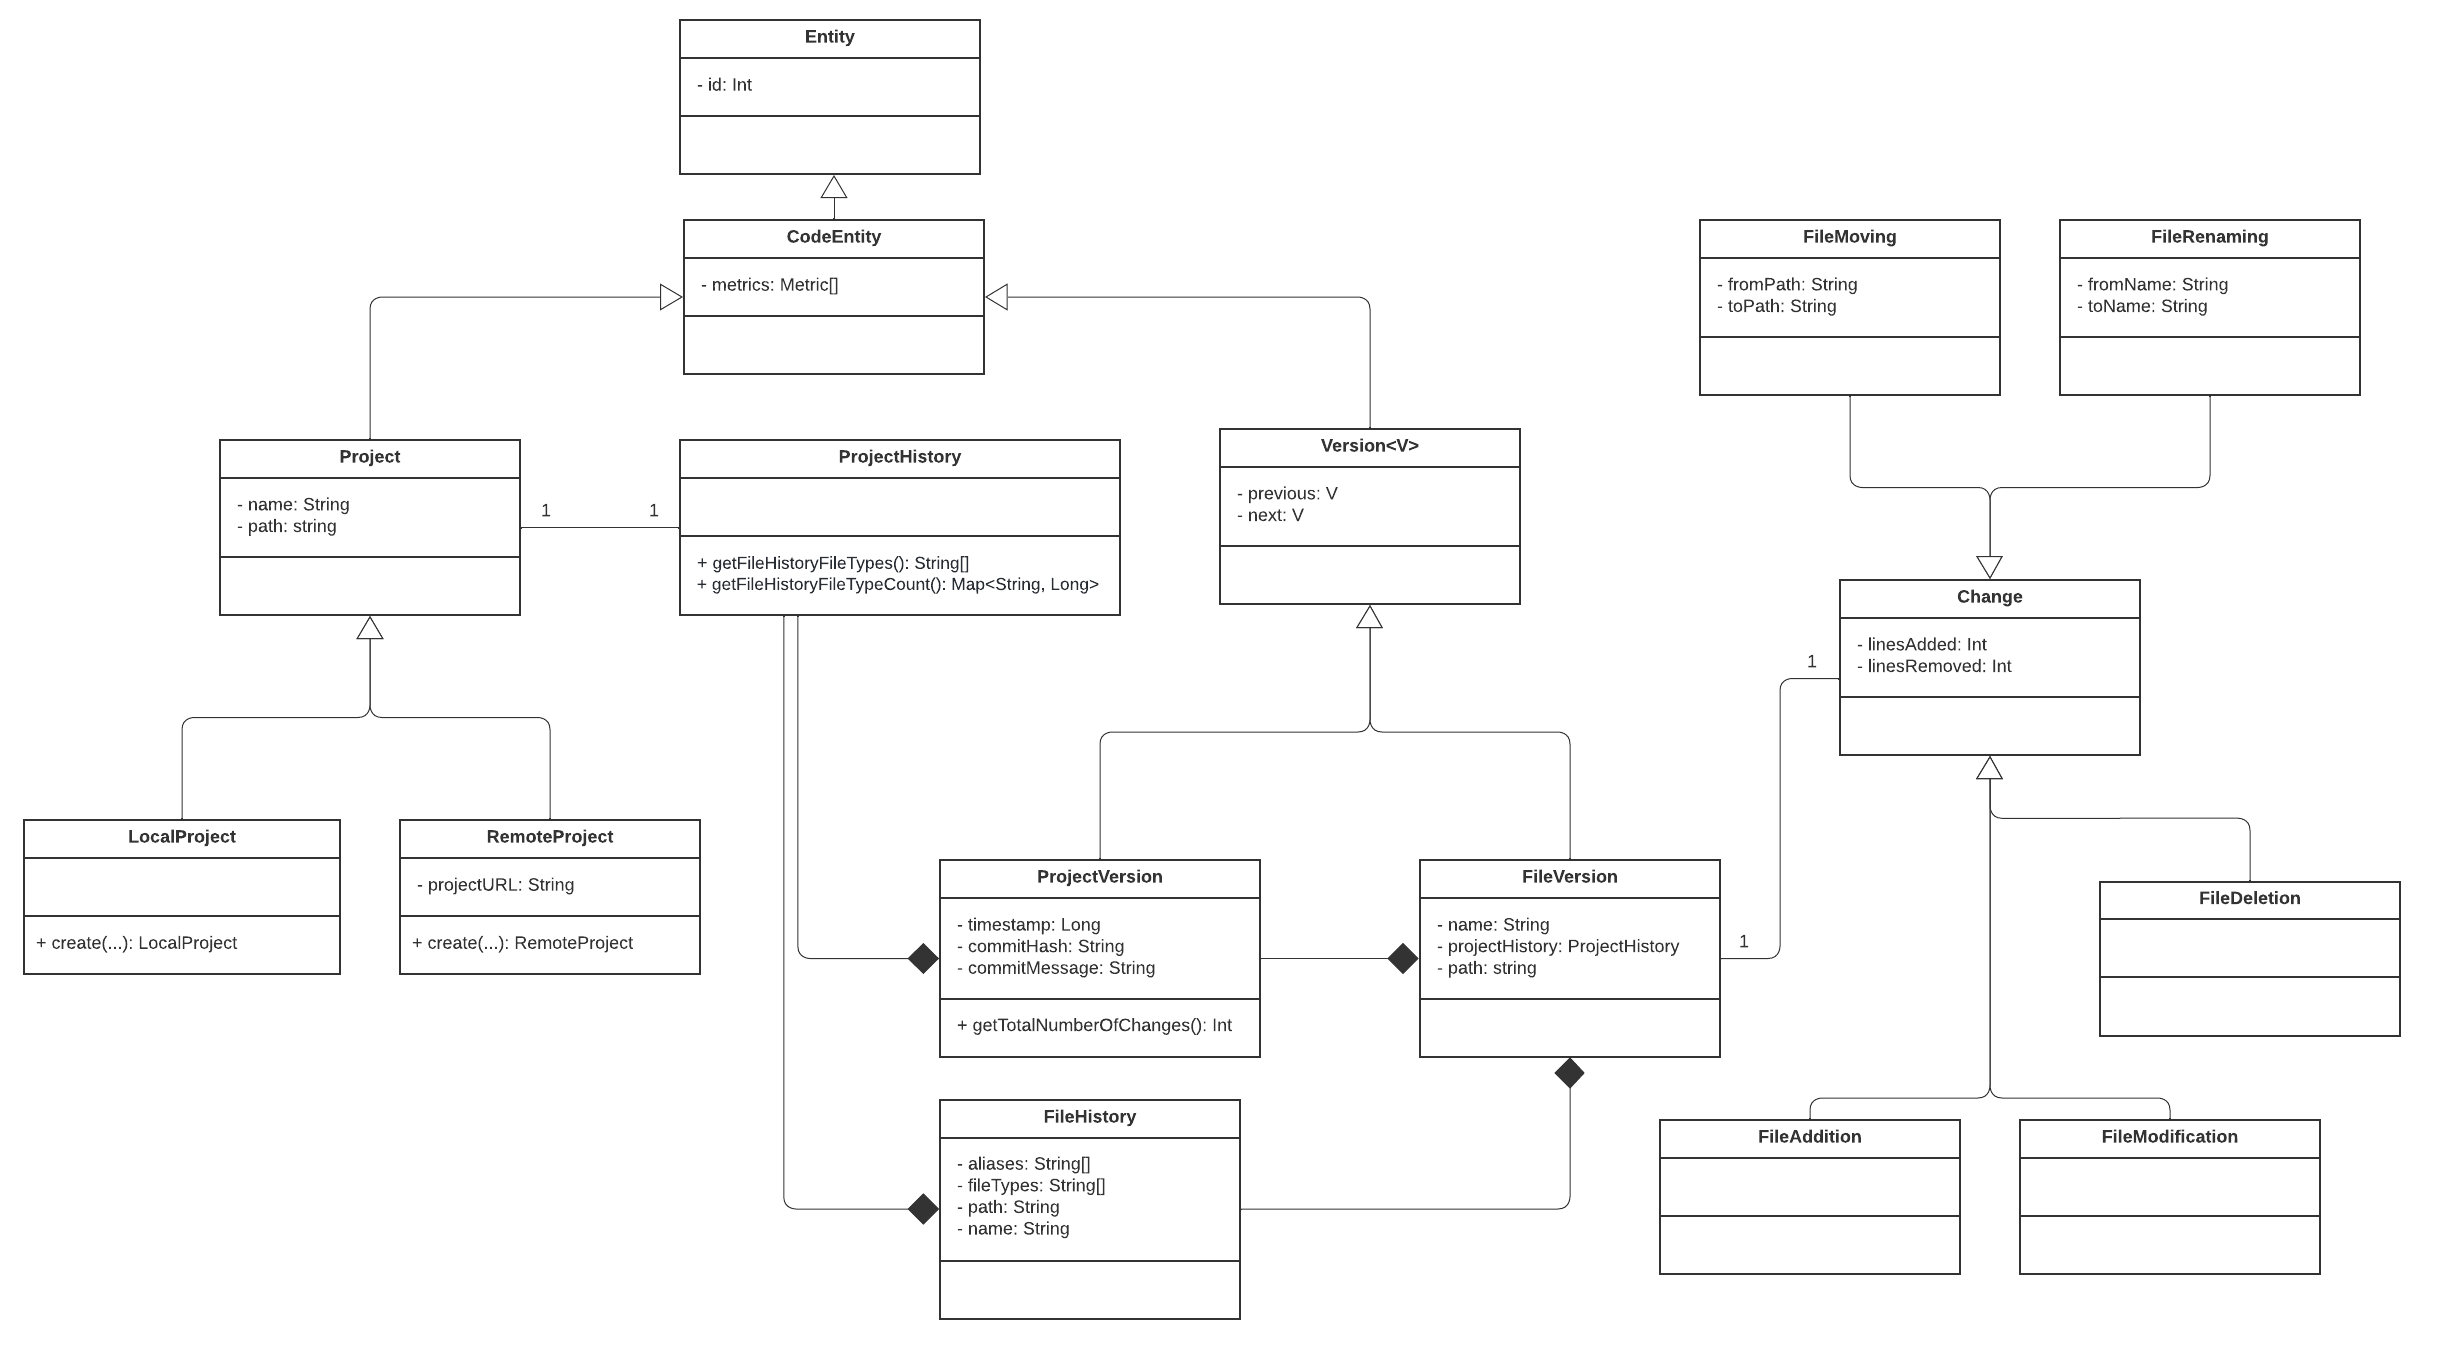
\includegraphics[width=\textwidth]{SYNClass.png}
    \caption{Class diagram of Project entities}
    \label{fig:SYNCLass}
\end{figure}

\subsection*{History}

Each project might hold a \textbf{ProjectHistory} object representing its history. 
The \texttt{ProjectHistory} class holds a group of ProjectVersion and a group of FileHistories. The \texttt{FileHistory} class has the following fields:
\begin{itemize}
    \item \texttt{aliases}: a list of paths related to the file. Usually, a single unique path identifies a file. However, since our approach tracks file moving and renaming, we store all the paths a file had throughout its evolution. In \autoref{sec:SYNAnalyzer} we further explain the importance of this field. 
    \item \texttt{fileTypes}: A set of Strings, each representing a type assigned to the file. 
    \item \texttt{path}: the path of the file. 
    \item \texttt{name}: the name of the file.
    \item \texttt{fileVersions}: a list of FileVersions related to this FileHistory. 
\end{itemize}
With the \texttt{Version<V>} class, we represent the state of an entity at a particular point in time. 
The generic parameter \texttt{V} is a constraint to ensure the consistency of the class with the previous and the subsequent versions. 

The \texttt{ProjectVersion} class is used to represent git commits; it defines the following fields: 
\begin{itemize}
    \item \texttt{fileVersions}: a list of FileVersions that are part of this commit.
    \item \texttt{timestamp}: expressed in seconds. 
    \item \texttt{commitHash}: hash of the commit generated by git when the commit was made and used to identify a commit uniquely. 
    \item \texttt{commitMessage}: the message written by the commit author when it was made. 
\end{itemize}
Extending the Version class, the ProjectVersion class also inherits the previous and next fields that could be used to navigate through the history. 
Finally, the \texttt{FileVersion} class has the following fields:
\begin{itemize}
    \item \texttt{parentProjectVersion}: the ProjectVersion holding this FileVersion instance. It retrieves the commit's related information, such as the timestamp or the message. 
    \item \texttt{change}: represents the action on that file. 
    \item \texttt{fileHistory}: represents the file being modified. 
\end{itemize}

In our approach, we identified five different types of changes. They were implemented by extending the \texttt{Change} class, as depicted in \autoref{fig:SYNCLass}. The \texttt{Change} class declares two fields, \texttt{linesAdded} and \texttt{linesRemoved}, each one representing the number of lines added and, in turn, removed. 
As extensibility was one of our design goals, a new change type can be implemented by extending this class.
For example, \texttt{FileMoving} and \texttt{FileRenaming} extend \texttt{Change} and specify two fields to track the path before and after a move or rename.



\subsection*{Analysis}
The Core provides abstract classes to standardize the exchange of analysis results. 
The first class that the model defines is \textbf{AnalysisWorkDescriptor}.
It is a holder of the information to instruct the analyzer on what it has to do. Namely, the project and the list of commits to be analyzed.
The reason for this implementation choice is to allow multiple threads to run in parallel analyses without analyzing the same commit numerous times. 
We described this approach in \autoref{s:EvolutionModel}


The \textbf{FileTypeManager} class is responsible for mapping a set of functions to file types. These functions are used to compute evolutionary metrics. We implemented the metrics presented in \autoref{s:EvolutionModel}. However, any external module could easily extend this set of functions. This choice allowed external components to increase the set of metrics computed in SYN. Therefore, the analysis can be customized to collect relevant metrics for a specific project. Once the function to extract a metric given a File is written, the developer must associate it with the corresponding file type. For example, if in the future an engineer wants to write an  Object-Oriented (OO) metric, such as the number of parents, they can create a function to compute it and associate the function to the OO.

Finally, the \textbf{ProjectAnalysisResult} class is used by an analyzer to return its results. This class makes a distinction between partial and total analysis results, allowing it to be used with the partial history retrieval approach defined in \autoref{sec:partialHistoricalRepr}. The fields declared in this class are:
\begin{itemize}
    \item \texttt{project}: the projects of the analysis.
    \item \texttt{analysisCompleted}: whether the analysis is partial or total.
    \item \texttt{timestamp}: the timestamp when the analysis was done. 
    \item \texttt{firstCommit}: the first commit considered in this analysis. 
    \item \texttt{lastCommit}: the last commit considered in this analysis. 
    \item \texttt{projectVersions}: a list of ProjectVersion founded during the analysis.
    \item \texttt{fileHistories}: a list of FileHistories created during the analysis.
    \item \texttt{fileVersions}: a list of FileVersions created during the analysis.
\end{itemize}

This module also provides an abstraction of the core concepts of the Git protocol. It defines the \texttt{GitProject}, \texttt{GitCommit} and \texttt{GitChange} classes, each representing a repository, a commit, and a change on a file respectively. 
Thanks to this choice, an external module can provide a way to retrieve data from a git repository without sharing internal classes or dependencies with other modules. 


\subsection*{View}
\label{s:view_impl}
In \autoref{s:3DRepr} we explained our visual approach. The \textbf{View} class defines how the visualization should be rendered. 
To display a repository's evolution, the user interface sequentially displays a list of AnimationFrames, each representing a state of the repository at a particular time. We designed the class \textbf{ViewAnimation} to define a frame of the view animation. This class has two properties:
\begin{itemize}
    \item \texttt{representedEntities}: a list of ProjectVersions whose data had been used to create that frame.
    \item \texttt{viewFigureList}: a list of ViewFigure, each representing a FileHistory in the view.
\end{itemize}

The \textbf{ViewFigure} class holds graphical properties to display a FileHistory: \texttt{position}, \texttt{color}, \texttt{height}, \texttt{shape}, \texttt{age}, \texttt{opacity}, and \texttt{size}.

These properties are computed when a \texttt{View} object is instantiated. A view is created with the user's preferences. 
For example, if the user wants a specific color for a particular action, like dark green for additions, we store this information in the \texttt{ViewSpecification} class. A \texttt{ViewSpecification} is the crucial element of each view. 
All the views are generated from a \texttt{ViewSpecification} instance. The list of available properties defined in a \texttt{ViewSpecification} are:
\begin{itemize}
    \item \texttt{versionGroupingStrategy}: the strategy to group commits and create AnimationFrames.
    \item \texttt{versionGroupingChunkSize}: the dimension of each group; it can be several commits or an amount of time. 
    \item \texttt{colorPalette}: the mapping of the FileVersion's actions to colors. 
    \item \texttt{agingGroupingStrategy}: the strategy group to define an age.
    \item \texttt{agingStepSize}: the dimension of each age; it can be the number of commits or the amount of time. 
    \item \texttt{agingSteps}: the number of available aging steps. 
    \item \texttt{mapperStrategy}: the strategy to compute the height of each entity once the metric's values are retrieved. For example, bucket strategy. 
    \item \texttt{mapperStrategyOptions}: optional properties of the mapper if needed. For example, the maximum height. 
    \item \texttt{mapperMetricName}: the metric's name that the mapper should consider before applying the selected MapperStrategy. 
    \item \texttt{showUnmappedEntities}: whether the view should display entities without the selected metric.
    \item \texttt{fileTypeShape}: the mapping to follow to associate a file type with a shape.
    \item \texttt{fileTypeOpacity}: the mapping to follow to associate a file type with an opacity level.
    \item \texttt{figureSize}: the size of each figure representing a file.
    \item \texttt{figureSpacing}: the space between each figure representing a file.
    \item \texttt{showDeletedEntities}: whether the view should display deleted entities.
    \item \texttt{withGround}: whether the view should include a ground element.
\end{itemize}

We defined an abstract class \textbf{PositionLayout} whose implementation specifies how entities should be laid out and a class \textbf{MapperStrategy} whose implementation specifies how the height of the entity is computed. The set of mapping functions is extensible. To implement a strategy a developer needs to implement an interface that defines two methods: \texttt{void generateStrategy(final List<String> values)} and \texttt{double mapValue(final String value)}. The mapping process is composed of two phases:
\begin{itemize}
    \item Generation phase: when the view is created, the method \texttt{generateStrategy} is called with all the values of the chosen metric. 
    \item Retrieve phase: when ViewFigure's height is retrieved. It is set as the return value of the function \texttt{mapValue}. 
\end{itemize}
\noindent
In our initial implementation, we provided five different mapping strategies:
\begin{itemize}
    \item LinearMapperStrategy: this strategy adopts a linear function to retrieve the height of a ViewFigure. 
    \item NormalizerMapperStrategy: during the generation phases, all the values are normalized in an interval between zero and one.

    \item BucketCountStrategy: during the generation phases, all the values are partitioned into buckets. This function calculates the number of buckets for a given value. This strategy allows the customization of the number of buckets that are created. By default, this value is set to 100. 
    \item BucketValueStrategy: relies on the BucketCountStrategy. During the generation, duplicate values are removed to equally distribute buckets.

    \item LinearBucketValueStrategy: relies on the BucketValueStrategy. During the generation phase, the maximum value of each bucket is recorded. Therefore, during the retrieved phase, it is used to make a liner proportion of the value and add them to the bucket number. For example, assuming that values of metrics are mapped to 100 buckets; the values $100, 200, 500$ are all mapped to the bucket $3$. Therefore when we need to map the number $100$ is mapped to $3 + 100/500 = 3.2$; in the same way, the value of $200$ is mapped to $3 + 200/500 = 3.4$ and the value of $500$ is mapped to $3 + 500/500 = 4$.
\end{itemize}



\section{CLI}
CLI is a command-line interface to interact with SYN.
\\
\textbf{Analysis commands}
\lstinline{syn analyze auto -p <project_id> -o <output_file> -t <thread_count>}\\
\\
This command is used to run an analysis with SYN. 
Given the project id, the system automatically creates \texttt{thread\_count} thread workers (5 by default), runs the analysis in parallel, and joins the results in the output file. The command ensures that each thread has a different git repository to work on. 


\lstinline{syn analyze join -o <output_file> <...analysis_file>}\\
\\
This command joins analysis results into a single output file.

\begin{lstlisting}
syn analyze manual -p <project_id> -g <git_repo_path>
    -rc <first_commit> -lc <last_commit> -o <output_file>
\end{lstlisting}

This command performs an analysis with SYN. It lets the developer choose the repository path and the first and last commits of the analysis. 
If the first commit is not specified, the analysis starts from the beginning of the history, and, in the same way, if the last commit is not specified, it completes with the end of the history. 


\begin{lstlisting}
syn analyze prepare -p <project_id>  -g <git_repo_path> 
    -wn <workers_number> -of <output_folder>
\end{lstlisting}

This command creates a new folder with many worker descriptors serialized into JSON files. These worker files are used to instruct the Analyzer on how it analyzes a project.
Based on the number of workers, the repository history is equally partitioned into chunks, each assigned to a worker. 


\lstinline{syn analyze worker -p <project_id> -g <git_repo_path> -w <worker_file> -o <output_file>}\\
\\
This command runs the analysis on a project given its worker file. 
Furthermore, here the user can specify the path of the repository on the local storage. This was done because a repository can be analyzed by only one worker at a time.

\textbf{Project commands}


\lstinline{syn project list}\\
\\
This command prints a list of available projects to the console.


\lstinline{syn project create -n <project_name> -p <project_location>}\\
\\
This command is used to create a project given its name and its location. The location could be either a path or an URL. 


\lstinline{syn project inspect -g <git_path> <project_id> <FileHistory_id>}\\
\\
This command inspects all the FileVersions of the indicated FileHistory. Furthermore, if the git repository is provided, SYN performs a double check to ensure that all the FileVersions were spotted. \
To do so, it exploits the output of the command \lstinline{git log --full-history -- <FileHistory_path>}, keeping attention if the FileHistory's path was changed (git cannot do that).


\lstinline{syn util csv <project_id> -o <output_file>}\\
\\
This command produces a CSV containing all the commits' tracked information of the selected project. 


\section{Analyzer}
\label{sec:SYNAnalyzer}
The Analyzer module implements the analysis approach described in \autoref{s:EvolutionModel}.
To walk through the git-tree, it uses a Java git adapter called JGit.\footnote{\url{https://www.eclipse.org/jgit/}} 
We extended the Git classes provided by the Core module, and created the \texttt{JGitProject}, \texttt{JGitCommit} and \texttt{JGitChange} classes. Their job is to call the JGit API and retrieve historical information. 


To run the analysis, we obtain first an \texttt{AnalysisWorkDescriptor}. 
The \texttt{JGitAnalysisWorkerDescriptorFactory} class partitions the commit tree and obtains a set of workers. 
\autoref{fig:historysplit} shows an example of a partition with three workers. First, the whole history of git is retrieved and stored in memory. Secondly, all the branches' commits are merged into a single list sorted by their timestamp. 
Then, the merge commits are removed since the changes recorded by them are duplicated and finally the resulting list is partitioned to match the requested number of workers. 
\begin{figure}
    \center
    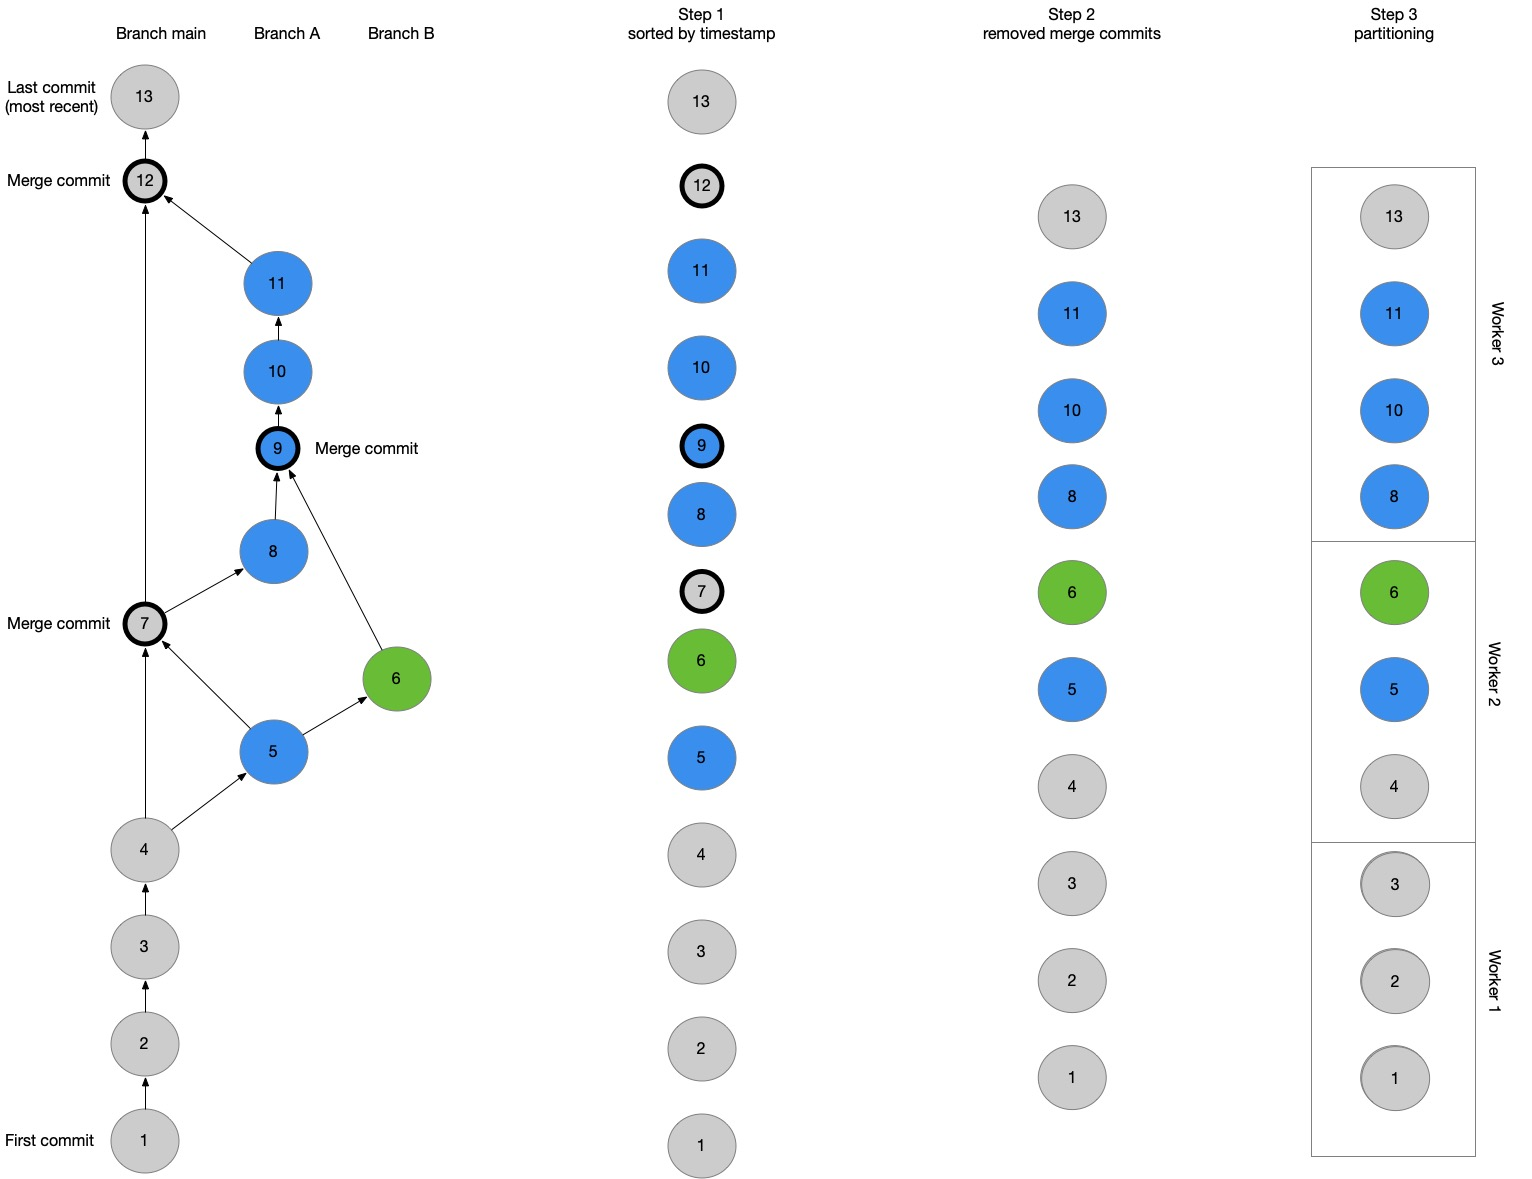
\includegraphics[width=\textwidth]{HistorySplit.jpg}
    \caption{Partition of the commit tree with 3 workers.}
    \label{fig:historysplit}
\end{figure}


The analysis process of a single worker contemplates the following steps:
\begin{enumerate}
    \item We call the method \texttt{runAnalysis} of the class \texttt{ProjectAnalyzer} with a worker descriptor and a project as an argument. 
    \item The analyzer reads the git path of the repository and instantiates a new \texttt{GitProject}. 
    \item A list of commits, specified in the worker, is retrieved from the \texttt{GitProject}.
    \item The first commit of the list is retrieved, and a new \texttt{ProjectVersion} is created with its details. 
    \item The analyzer runs the checkout command of git to restore the version of the system at the one specified by the commit. 
    \item The analyzer retrieves a list of modified files. 
    \item For each modified file, the analyzer creates a new \texttt{FileVersion}, links it with the corresponding  \texttt{ProjectVersion} and \texttt{FileHistory} (creates it if it does not exist yet), and finally extracts all the evolutionary metrics expected for that file type.
    \item Once all the modified files are analyzed, the analyzer repeats steps 5, 6, and 7, considering the subsequent commit of the list each time. 
    \item Once all the commits are analyzed, the analyzer returns the results as a \texttt{ProjectAnalysisResult} object. 
\end{enumerate}


The analyzer can parallelize with multiple workers the analysis of large repositories. Each worker produces a \texttt{ProjectAnalysisResult} that represents a partial history. To obtain the entire history of the repository, we join all partial analysis results. 
In SYN, each entity is identified by an id. 
The order in which entities are created is important because we visually sort entities based on their creation timestamp. 
Therefore, consistency between ids of FileHistories is necessary for the join algorithm.
We said that each analysis result has a list of \texttt{FileVersions}, a list of \texttt{ProjectVersions} and a list of \texttt{FileHistories}. 
Analyzers are not meant to communicate with each other. Therefore they work in isolation, like in a sandbox. 
When we join the results, the concatenation of the \texttt{FileVersions} or the \texttt{ProjectVersions} is not a problem when the historical sequence is respected. 
These objects are mutually independent of each other.
The challenge comes with the \texttt{FileHistories}. When the analyzer spots a file, if it was not discovered yet, it creates a new \texttt{FileHistory} with a unique id. 
This sounds like a problem with merging because we might consider the same file twice. In other words, we have an issue linking FileHistories between analysis results.
Assuming for a moment that we do not have this obstacle, another situation might happen, more complicated than the previous one.
 
If in the middle of two analysis results, a file changed its path, in the first analysis, we have an entity with the old path, 
and in the second analysis, we have an entity with a new path. 
Unless we would not keep track of all the possible paths of an entity, it is impossible to reconstruct a connection between these two files. 
This is the reason that brought us to add the \texttt{aliases} field in the \texttt{FileHistory} class. 
In the join algorithm we developed, we employ a map to keep track of FileHistories.
As a result, the file has a different id in any analysis result, guaranteeing consistency among FileHistories. Furthermore, we can ensure the absence of duplicates in the newly built repository history. 

We present an algorithm that takes as input a list of already discovered FileHistories and a \texttt{ProjectAnalysisResult}, and it returns a dictionary.
This dictionary is used to map partialFileHistories, the FileHistory of an analysis result, to definitive FileHistories, which are part of the entire history of the repository. 
To obtain this map, it uses the following strategy:
\begin{enumerate}
    \item If the last alias of a definitiveFileHistories is equal to the first alias of a partialFileHistory, then they represent the same file.
    \item If in the partialAnalysisResult there is more than one FileHistory with the same first alias, only the first is mapped to a definitiveFileHistories, and the other partialAnalysisResult are mapped to a new FileHistory.
    \item If a partialFileHistory has not matched an alias with a previously created definitiveFileHistories, then it represents a new definitiveFileHistories.
\end{enumerate}

% \begin{algorithm}
%     \caption{Algorithm to create a mapping between partialFileHistories and definitiveFileHistories}
%     \label{alg:cap}
%     \begin{algorithmic}[1]
        
%     \State $partialToDefinitiveMap \gets new Map()$
%     \State $partialAliasToFileHistory \gets new Map()$
%     \State $newFileHistories \gets new List()$
%     \end{algorithmic}
% \end{algorithm}

\begin{algorithm}
    \caption{Algorithm to create a mapping between partialFileHistories and definitiveFileHistories}
    \begin{algorithmic}[1]
    \Procedure{PartialToDefinitiveFH}{$projectAnalysisResult, partialFileHistories$}
        \State $partialToDefinitive \gets Map()$
        \State $partialAliasToFH \gets Map()$ \Comment{Strategy 1}
        \State $unmappedPartialFileHistories \gets List()$  \Comment{Strategy 2}
        \ForAll{partialFH in partialFileHistories}
            \State $firstAlias \gets partialFH.aliases[0]$
            \If{$!partialAliasToFH.has(firstAlias)$}
                \State $partialAliasToFH.set(firstAlias, partialFH)$  \Comment{Strategy 1}
            \Else
                \State $unmappedPartialFH.append(partialAliasToFH)$  \Comment{Strategy 2}
            \EndIf
        \EndFor

        \ForAll{definitiveFH in projectAnalysisResult} \Comment{Strategy 1}
            \State $lastAlias \gets definitiveFH.aliases[definitiveFH.length - 1]$
            \If{$partialAliasToFH.has(lastAlias)$}
                \State $partialFH = partialAliasToFH.get(lastAlias)$
                \State $definitiveFH.path = partialFH.path$
                \State $definitiveFH.aliases.addAll(partialFH.aliases)$
                \State $partialToDefinitive.set(partialFH, definitiveFH)$
                \State $partialAliasToFH.remove(lastAlias)$
            \EndIf
        \EndFor

        \State $unmappedPartialFH.addAll(partialAliasToFH)$ \Comment{Strategy 3}
        \ForAll{partialFH in unmappedPartialFH} 
            \State $definitiveFH = FileHistory(partial.name, partial.path)$
            \State $definitiveFH.aliases = partialFH.aliases $
            \State $partialToDefinitive.set(partialFH, definitiveFH)$
        \EndFor
        \State \textbf{return} $partialToDefinitive$
    \EndProcedure
    \end{algorithmic}
\end{algorithm}


\section{Server}
The server is responsible for providing the analysis results, in an intermediate language between the 
front-end (Visual Inspector). We developed the server with Spring Boot, a popular Java application framework.\footnote{\url{https://spring.io/projects/spring-boot}}

\subsection*{GraphQL API} 
The server module provides a set of GraphQL\footnote{\url{https://graphql.org/}} endpoints to retrieve information from SYN. 
GraphQL is a data query and manipulation language for APIs. It also provides the runtime engine for fulfilling the queries.
This is an advantage compared to a REST API because, instead of always returning a predefined set of data, GraphQL only returns the needed information, making the communication more effective. 
In GraphQL, endpoints are divided into queries and mutations. Queries retrieve data, while mutations create or alter data. In the rest of this section, we present the mutations and queries defined in our GraphQL API.


\textbf{Mutations}
\texttt{createProject(projectName: String!, projectLocation: String!): Project} \\
creates and initiates the analysis of a new project.
It takes as parameters the project name and its path on the local machine or the URL as a String. 

\textbf{Queries}
\texttt{projectList:  [PartialProjectInformation]!} \\ 
is used to retrieve a list of projects. For performance reasons, only the name and the id of a project can be retrieved. 
\bigbreak
\texttt{view(projectId: Int!, viewSpecification: ViewSpecificationInput!): View} \\
returns a view of the project identified by \texttt{projectId}, built following the directives specified in the \texttt{viewSpecification} object. 
This query returns an object representing a view; thus, it has all the fields described in \autoref{s:view_impl}. 
\bigbreak
\texttt{partialView(projectId: Int!, viewSpecification: ViewSpecificationInput!, viewAnimationId: Int): View} \\
returns a view with the next 100 AnimationFrames starting from \texttt{viewAnimationId}. 
This endpoint was created to improve the clients' performance. If the viewSpecification expected too many animations, the resulting view would be a bottleneck for the client.
With this endpoint it can still retrieve the view, and then animation can be lazily loaded when they are required. 
\bigbreak
\texttt{fileHistory(projectId: Int!, fileHistoryId: Int!): FileHistory} \\
retrieves the FileHistory identified with \texttt{fileHistoryId} of the project with \texttt{projectId}.
\bigbreak
\texttt{projectVersions(projectId: Int!, projectVersionsId: [Int]!): [ProjectVersion]!} \\
retrieves the ProjectVersion identified with \texttt{projectVersionsId} of the project with \texttt{projectId}.
\bigbreak
\texttt{groupingPreview(projectId: Int!, viewSpecification: ViewSpecificationInput!): Int} \\
this endpoint computes the number of AnimationFrames created with the given \texttt{viewSpecification}.
\bigbreak
\texttt{fileTypeCounter(projectId: Int!): [FileTypeCounter!]!} \\
returns a list for each file type with the number of occurrences in the project \texttt{projectId}.
\bigbreak
\texttt{fileTypeMetrics(projectId: Int!, fileTypeFilter: [String]): [FileTypeMetrics!]!} \\
returns a list for each file type with its metrics. Only the file types in the \texttt{fileTypeFilter} list are considered. 

\clearpage
\begin{figure}
    \center
    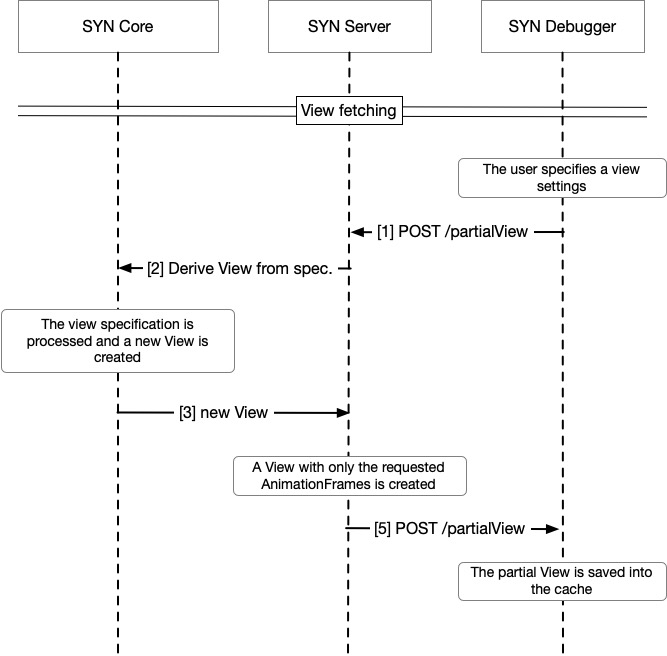
\includegraphics[width=0.7\textwidth]{ServertClientFlow.jpg}
    \caption{Example of the process of retrieving a view through GraphQL}
    \label{fig:ServertClientFlow}
\end{figure}


\autoref{fig:ServertClientFlow} explains how a View is retrieved through a GraphQL endpoint with a sequence diagram. Once the client, in this case, Visual Inspector, specified a \texttt{viewSpecification}, it makes a POST request to the 
\texttt{partialView} endpoint with the \texttt{projectId}, the \texttt{viewSpecification} and the \texttt{viewAnimationId} of the AnimationFrame. The Server module, in turn, makes the same request to the Core module. A new View is created and retrieved from Server. It is modified to include only the AnimationFrames requested from the client. When the partialView is computed, it is returned to the client. 


\section{Visual Inspector}
\label{s:SYNDebugger}

The Visual Inspector module is a web application to interact with SYN, written with React.js, a popular JavaScript framework. 
The visualization is based on Babylon.js, an open-source 3D library. 
It provides different customizations for the visualization, such as the entities' shape and color. 
These customizations are sent to the back-end server through a {\em view specification} file as shown in \autoref{fig:ServertClientFlow}. 

The primary purpose of this application is to debug the view and explore all the possible visualization combinations of a system.
The main page, shown in \autoref{fig:SYNUIList}, holds a list of projects analyzed with SYN.

\begin{figure}
    \center
    
\includegraphics[width=\textwidth]{SYNUI-List.png}
    \caption{SYN Visual Inspection main page}
    \label{fig:SYNUIList}
\end{figure}

\subsection*{Project setup}
When a project is selected, the UI searches for a viewSpecification object in the web browser's local storage. 
If it is not present, the module shows the project setup. At the end of the setup, all the preferences selected are saved. 
The project setup is a wizard to configure a project's visualization, composed of five main steps as follows:
\begin{itemize}
    \item Component selection: where the user can select which kind of file type must be considered in the visualization. To help the user, SYN presents the project's file types distribution.
    \item Grouping version strategy: the user can choose how commits are grouped to create AnimatioFrames.
    \item Figure settings: to customize the shape, metrics, and opacity of each file type. The user can also choose which strategy must be used to compute the entity's height. 
    \item View color: to customize the color of each git action and how aging must act. 
    \item View settings: to customize general settings such as the speed of the visualization, shadows, or whether deleted entities should be visualized. 
\end{itemize}

\subsubsection*{Component selection}
\autoref{fig:SYNUIsettings1} presents the first step of the project setup. It shows a list of cards, each representing a file type. 
We can break the visualization area into two parts: on the top, there are two cards to represent binary files and text files. 
The sum of these two represents the total number of FileHistories in the system because each file must be either textual or binary. 
The bottom part shows the cards for the file types identified in the project. For example, if a file is named \quotes{foo.java} the JAVA card in this area represents it. 
The cards are sorted in descending order by their number of occurrences. This view considers all the file types present in the system. To show the complete list, users have to click on the \quotes{show more} button.

\begin{figure}
    \center
    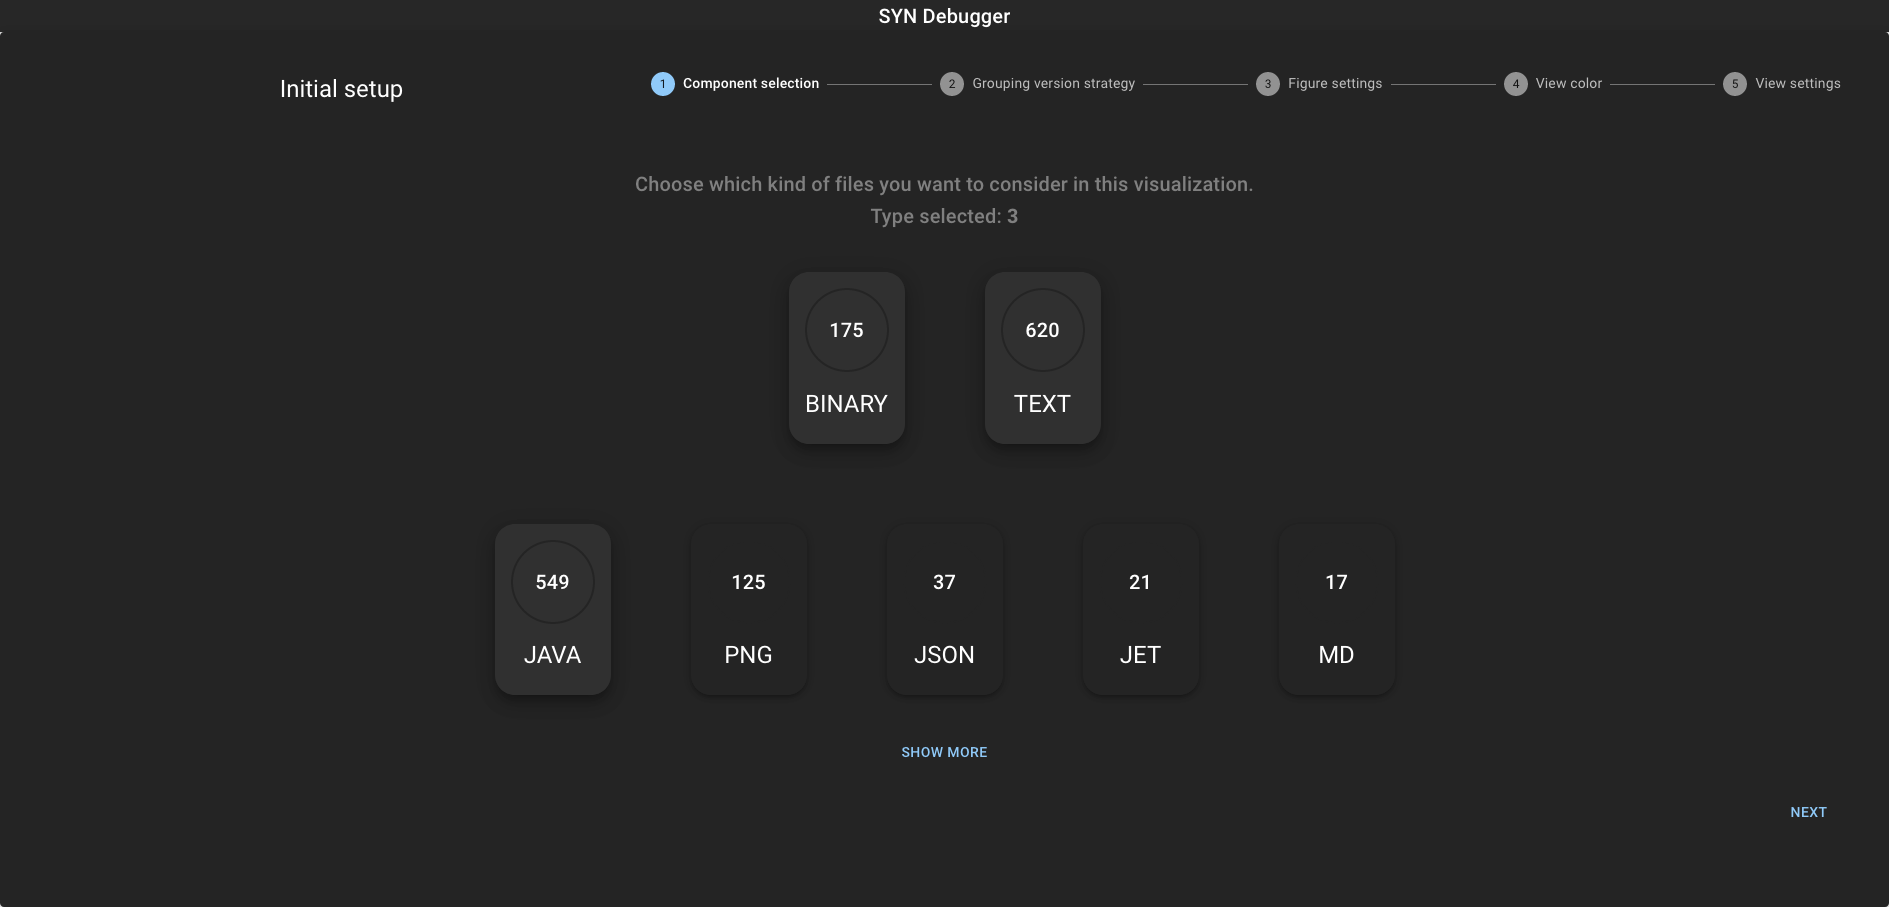
\includegraphics[width=\textwidth]{SYNUI-settings1.png}
    \caption{Project setup: component selection}
    \label{fig:SYNUIsettings1}
\end{figure}


\subsubsection*{Grouping strategy}
\autoref{fig:SYNUIsettings2} shows the second configuration step. It allows the user to choose how SYN groups ProjectVersions. 
Following what we have presented in \autoref{s:3DRepr}, we provide two strategies to group ProjectVersions:
\begin{itemize}
    \item by commits: we create an AnimationFrame every $n$ commits. 
    \item by timestamp: we create an AnimationFrame every $n$ seconds. 
\end{itemize}

To ease the selection of the timestamp strategy, instead of manually computing the width of the time window, the user must only specify an amount and its time unit (i.e., hour, day, week, month, year). After the selection, the UI shows a preview of the grouping strategy to give an idea of how many animations are created with the selected settings. 
\begin{figure}
    \center
    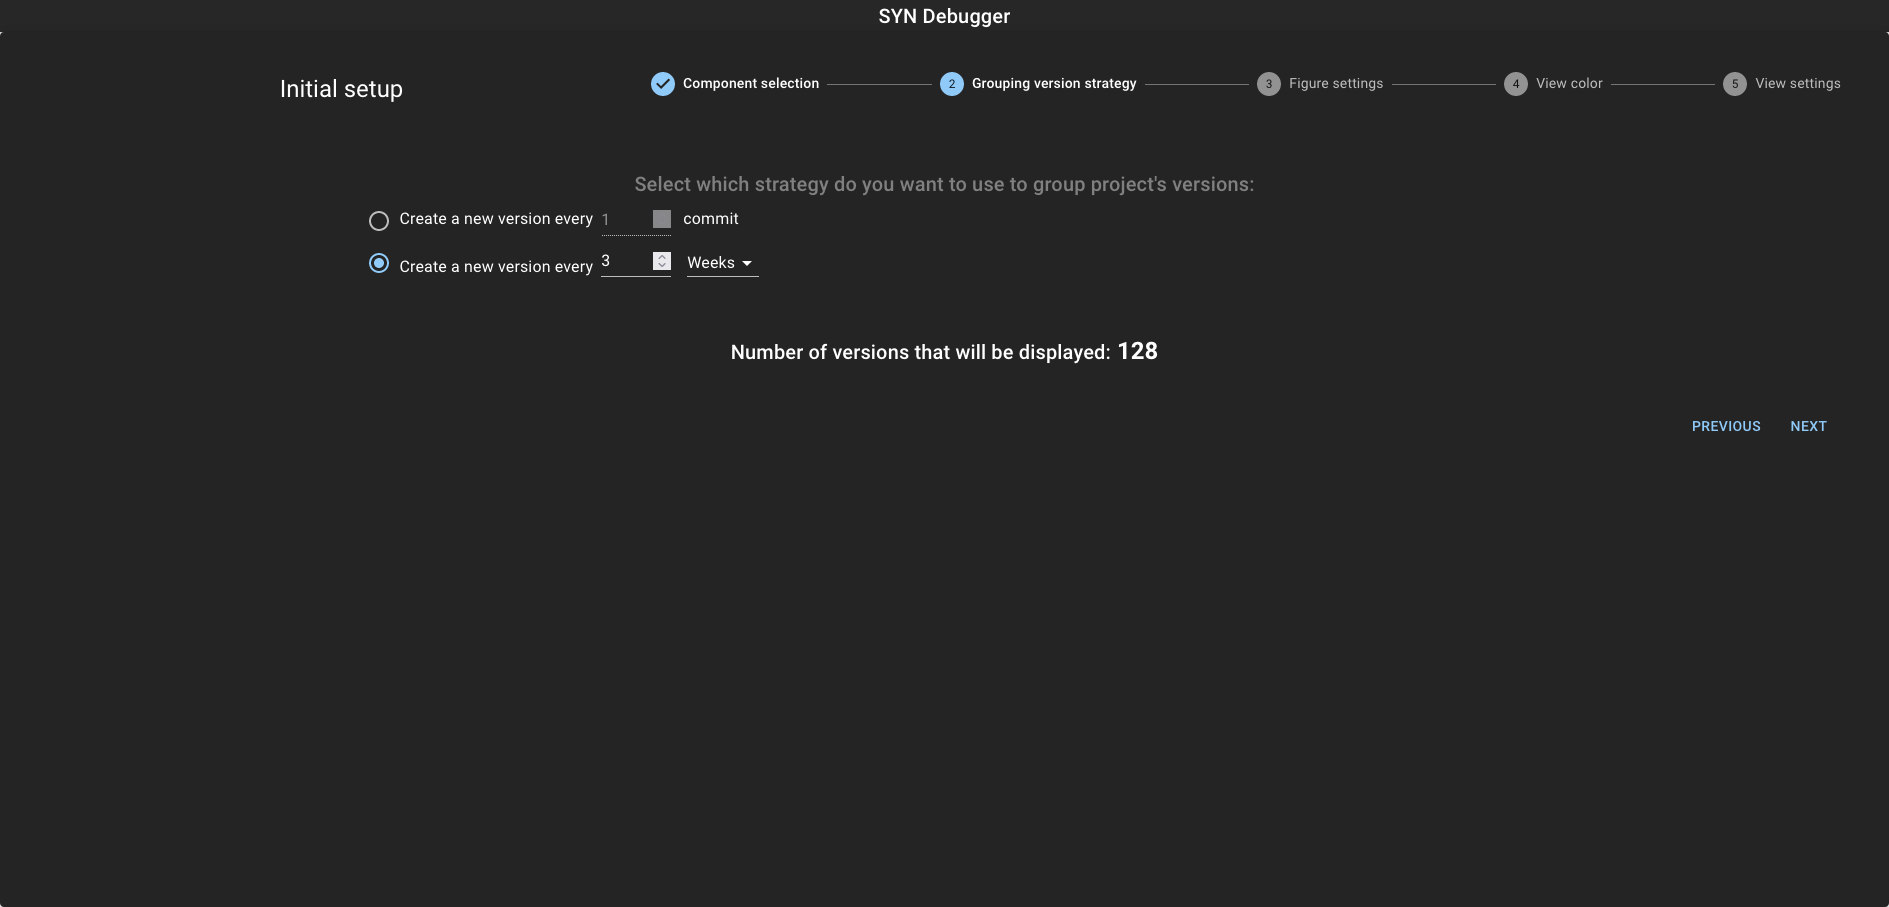
\includegraphics[width=\textwidth]{SYNUI-settings2.png}
    \caption{Project setup: grouping strategy}
    \label{fig:SYNUIsettings2}
\end{figure}

\subsubsection*{Figure settings}
The third step of the setup is shown in \autoref{fig:SYNUIsettings3}. It allows the user to express graphical preferences. 
The view creates a card for each file type selected in the \quotes{Component selection} step.
The user can customize each card with the followings:
\begin{itemize}
    \item Metrics: a list of metrics that should be visualized when a file is selected. 
    \item Shape: in our visualization, we implemented five shapes: box, triangular, cone, sphere, and cylinder. 
    \item Opacity: to control the transparency of each file type.
\end{itemize}

The user can also configure which metrics and mapper strategies determine the height of entities and the maximum height of the entities. 
The list of available metrics for the mapper comprises the metrics selected for each file type.
The UI has a checkbox to specify whether FileHistories that do not have the selected metric should be rendered or not. 

With all the settings available on this page, the user has complete control over how FileHistories are rendered. 
There are many possible combinations. For example, if we want a visualization that distinguishes between Java, text, and binary files, we can use settings shown in \autoref{fig:SYNUIsettings3}. It specifies a different shape for every file type, keeping the maximum opacity level for all of them. Furthermore, the height is computed with a bucketValueStrategy that works with the SLOC metric. As a consequence, only Java files have a height in this visualization. File types that don't have the mapper metric are called \quotes{unmapped entities}, and their height will be fixed. 



\begin{figure}
    \center
    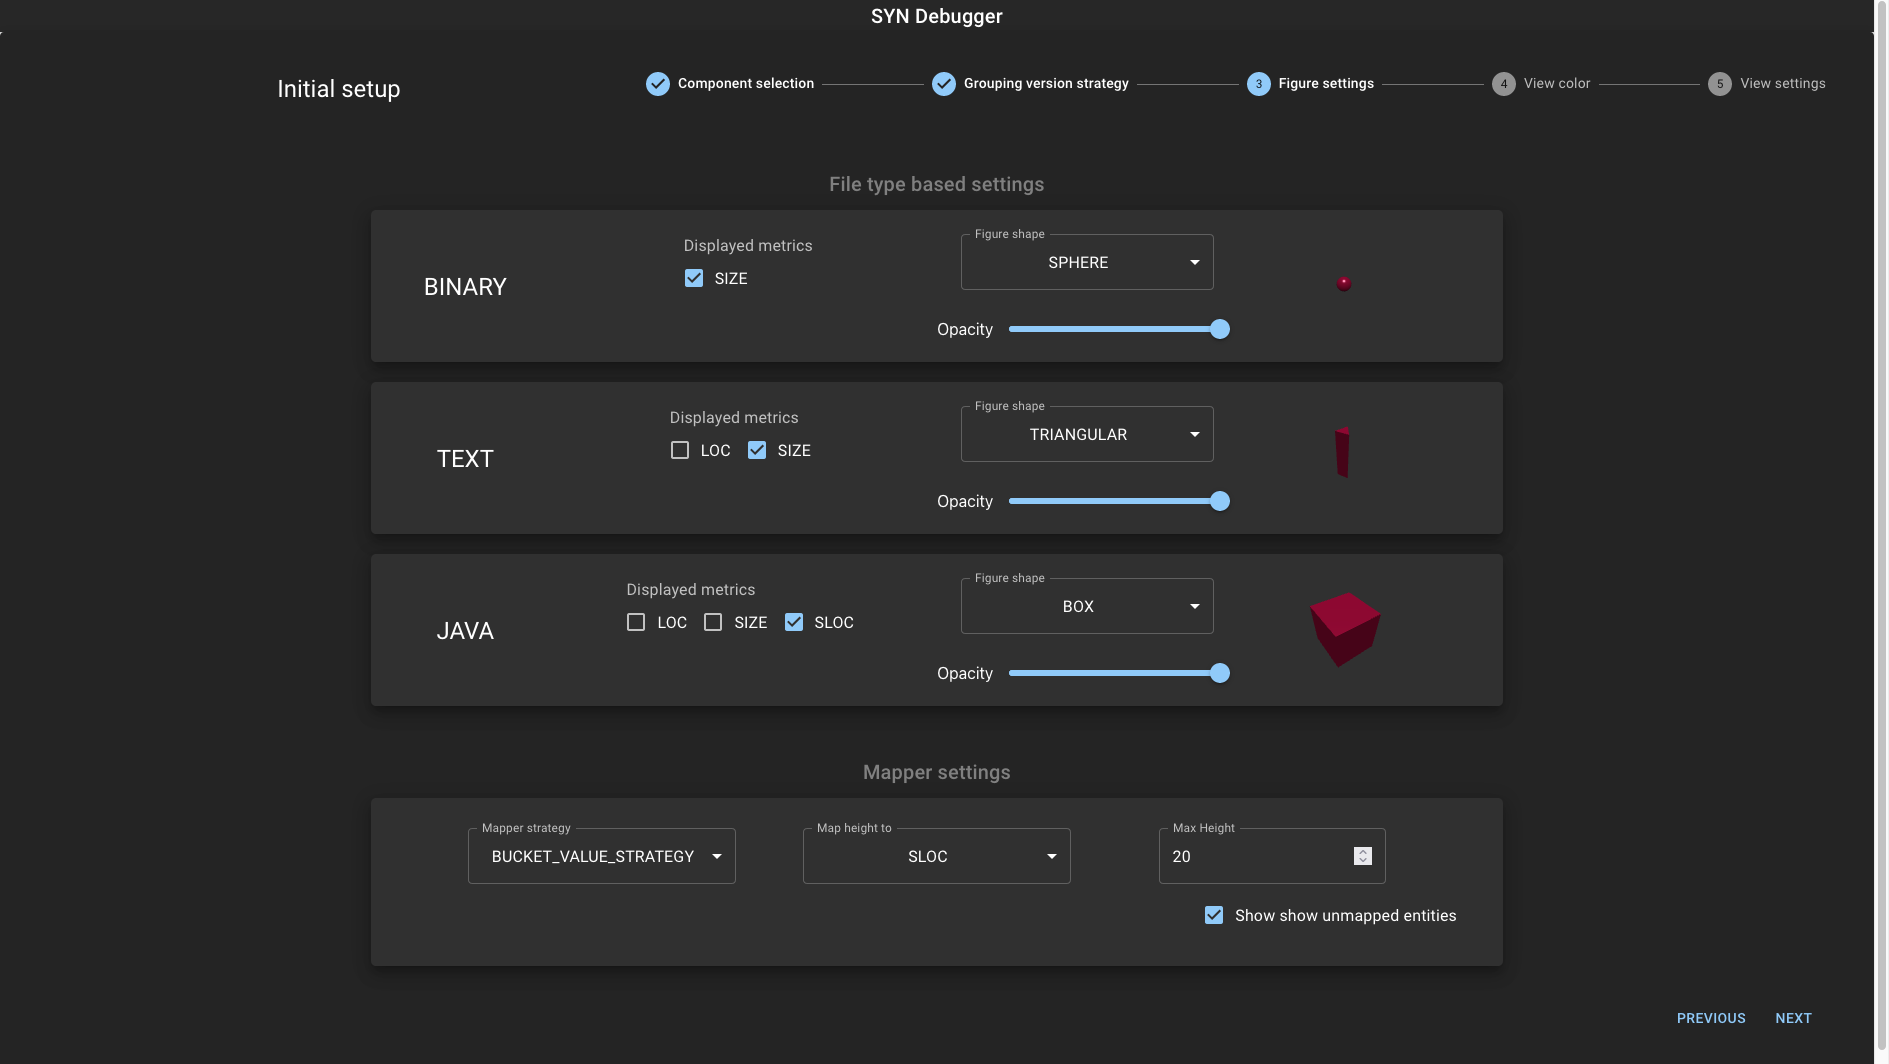
\includegraphics[width=\textwidth]{SYNUI-settings3.png}
    \caption{Project setup: figure settings}
    \label{fig:SYNUIsettings3}
\end{figure}

\subsubsection*{View color}

\autoref{fig:SYNUIsettings4} shows the last setup step. It configures the remaining general UI preferences as follows:
The user controls the way how aging is computed. 
As with grouping versions, aging can be done following two possible strategies: one by timestamp and one by commits. 
The color transition is linear. Therefore, the user can choose the number of steps between the original color of the entity and the base color. 

Finally, each action has a distinct original color, customizable for the user. The color palette used by default is shown in \autoref{fig:SYNUIsettings4}.

\begin{figure}
    \center
    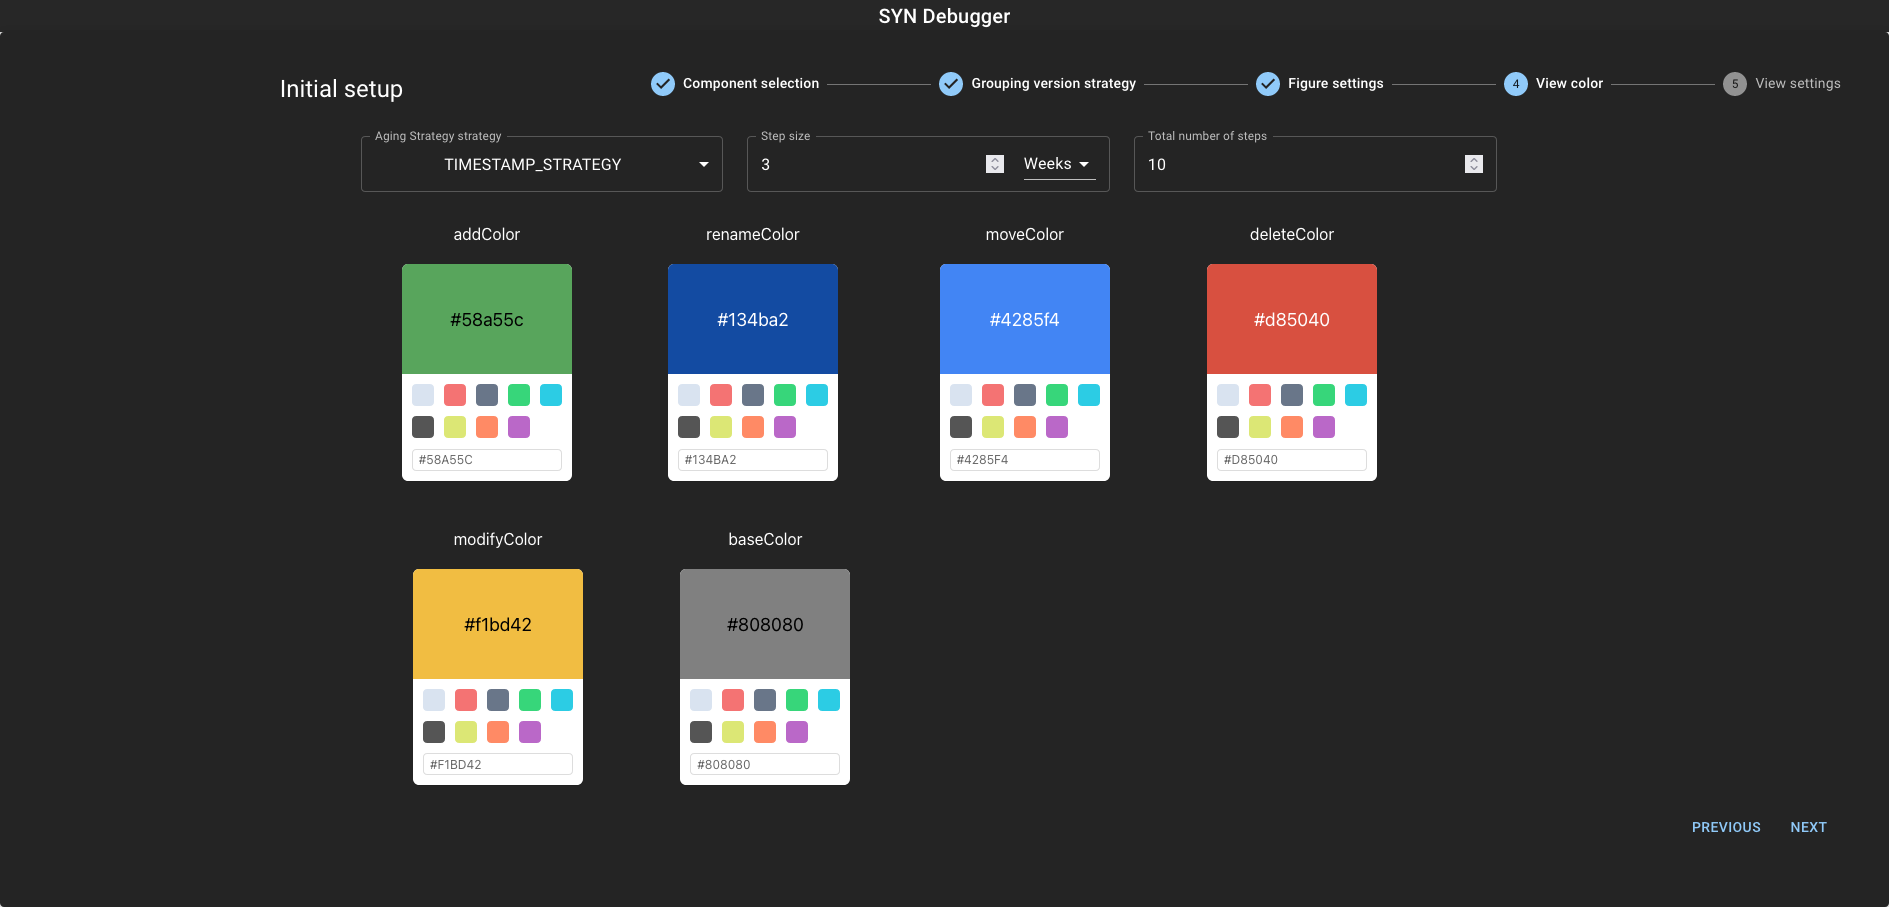
\includegraphics[width=\textwidth]{SYNUI-settings4.png}
    \caption{Project setup: view color}
    \label{fig:SYNUIsettings4}
\end{figure}

\subsubsection*{View settings}
The last step of the setup, shown in \autoref{fig:SYNUIsettings5}, allows the user to express general preferences about the behavior of the UI.

\begin{itemize}
    \item Show VR Button: enables the full immersion experience that must be enjoyed with a VR headset. 
    \item Keep deleted entities: keeps deleted entities in the visualization. By default, these are not displayed. 
    \item Show debug layer: makes the 3D engine's debugger visible. 
    \item Auto screenshot: a screenshot of the visualization is generated with text indicating the time of the last commit included in the displayed AnimationFrame.
    \item Shadows: enables the shading of entities. 
    \item Animation switching speed: the amount of time between rendering one animation and another when the autoplay mode is activated. 
\end{itemize}

\begin{figure}
    \center
    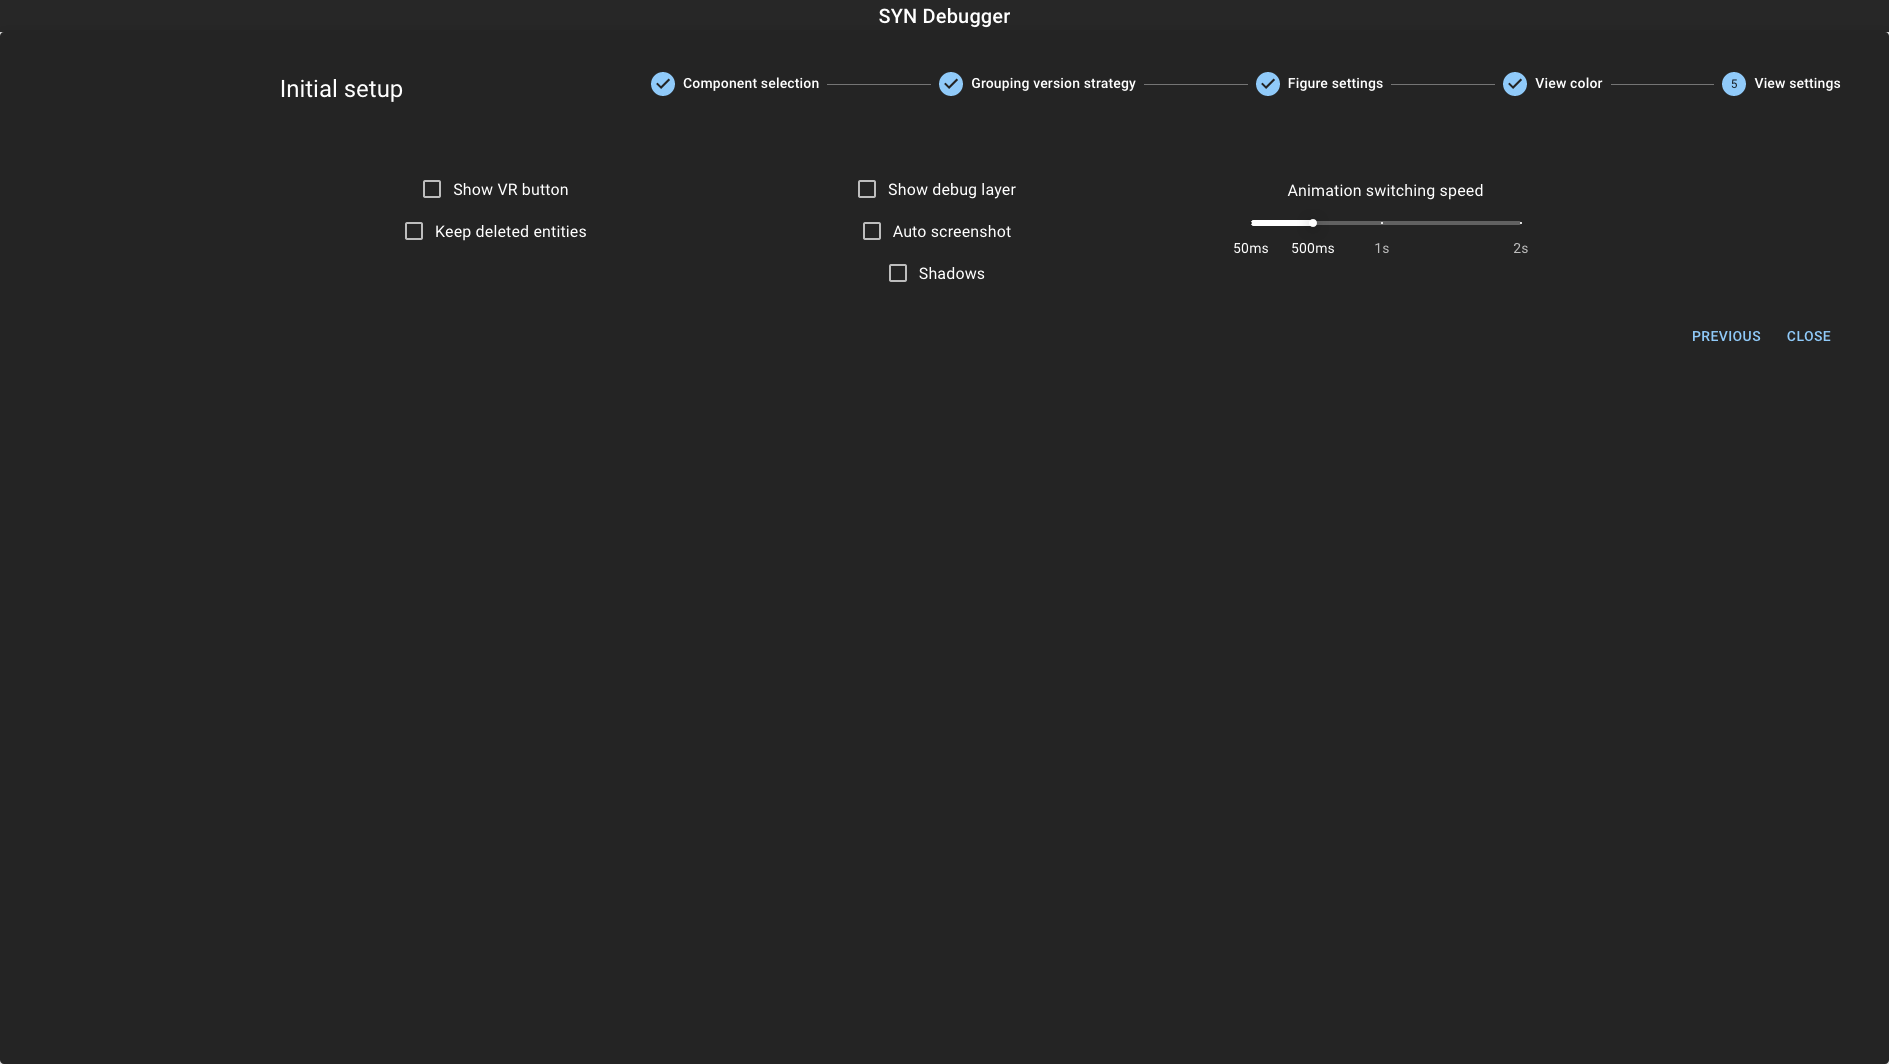
\includegraphics[width=\textwidth]{SYNUI-settings5.png}
    \caption{Project setup: view settings}
    \label{fig:SYNUIsettings5}
\end{figure}

\subsection*{Project visualization}
After having specified all the visualization preferences, they are stored in the web browser's local storage. 
The UI can retrieve a view from the backend server, given the project id and the view specification. 

Initially, it calls the \texttt{partialView} query provided by the Server module. Once it gets the response, the visualization of the first AnimationFrame is automatically loaded. 
A pre-fetcher mechanism was also implemented, it works as follows: once half of the retrieved AnimationFrames have been displayed; it lazily requests a new partialView containing all the following AnimationFrames of the currently displayed view. 
In this way, the jump between a partialView and another is not subjected to network timing issues because the partial view was already prefetched. 


The initial display of the view is represented in \autoref{fig:fileHistories}. The visualization settings of this view are:
\begin{itemize}
    \item Version grouping strategy: timestamp, three weeks
    \item Color palette: default
    \item Aging: timestamp, three weeks with ten steps
    \item Height mapper: BucketValueStrategy on SLOC
    \item Deleted entities are not shown
    \item All the entities have the same shape and opacity
    \item All the available metrics are selected for each file type. 
\end{itemize}

The main visualization area can be broken down into four parts: 
In box A, a 3D environment displays FileHistories on a virtual plane. The view angle and the zoom level of the camera can be controlled with the mouse. 
In box B, we have a card with general information about the project visualization. 
This card includes the project's name, the animation number, the dates of the animation frame, and its commit list. The slider shows the overall progress of the display, two buttons to jump to the subsequent or previous animation, and finally, one button to jump to the following animation with the time interval previously set. 
All the preferences specified during the project setup can be changed by clicking on the three dots in the top right corner.
In box C, we have a card to inform the user of the number of entities the UI renders. 
And finally, box D appears when an entity is selected with the mouse. 
It shows more details of the entity as follows:
\begin{itemize}
    \item the name and the current path of the entity. The current path is the entity's path in the last commit of the displayed animation frame. 
    \item a table filled with all the metrics retrieved on the last commit of the displayed animation frame. The list of metrics is filtered based on the project setup. 
    \item a table filled with all the FileVersions associated with the selected FileHistory. It shows the commit hash and the action made on that commit for each FileVersion. If the project is hosted on GitHub, when the user clicks on the commit hash, the Visual Inspector opens a new tab with the code of the class at that revision. A tooltip with commit information appears if you hover on an action with the mouse. 
    \item on right-click, a contextual menu gets displayed (box E). With this contextual menu, one can jump on GitHub to see the raw file in the last commit of the currently displayed animation. 
\end{itemize}

\autoref{fig:deletedshadow} provides another visualization example where deleted entities are shown in the visualization, and the shadows are displayed. 

\begin{figure}
    \center
    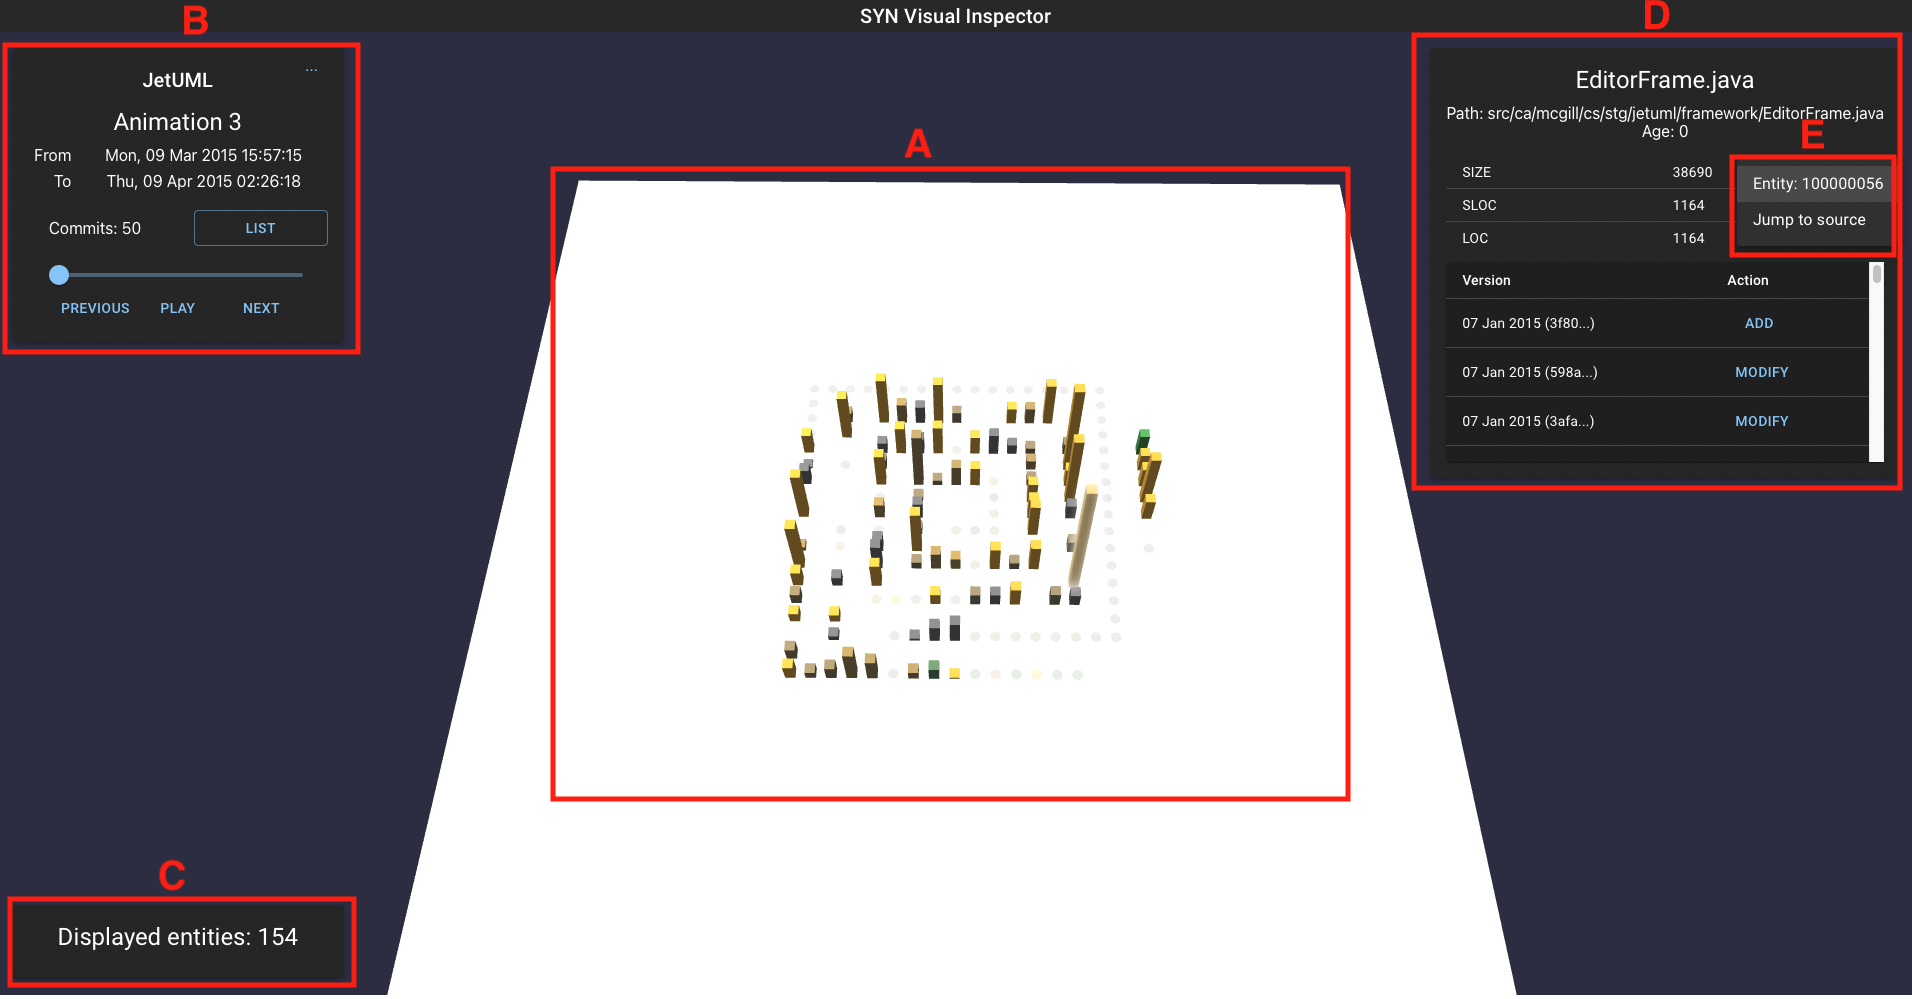
\includegraphics[width=\textwidth]{SYNUI-fileHistory2.png}
    \caption{Visualization of JetUML with the default settings.}
    \label{fig:fileHistories}
\end{figure}

\begin{figure}
    \center
    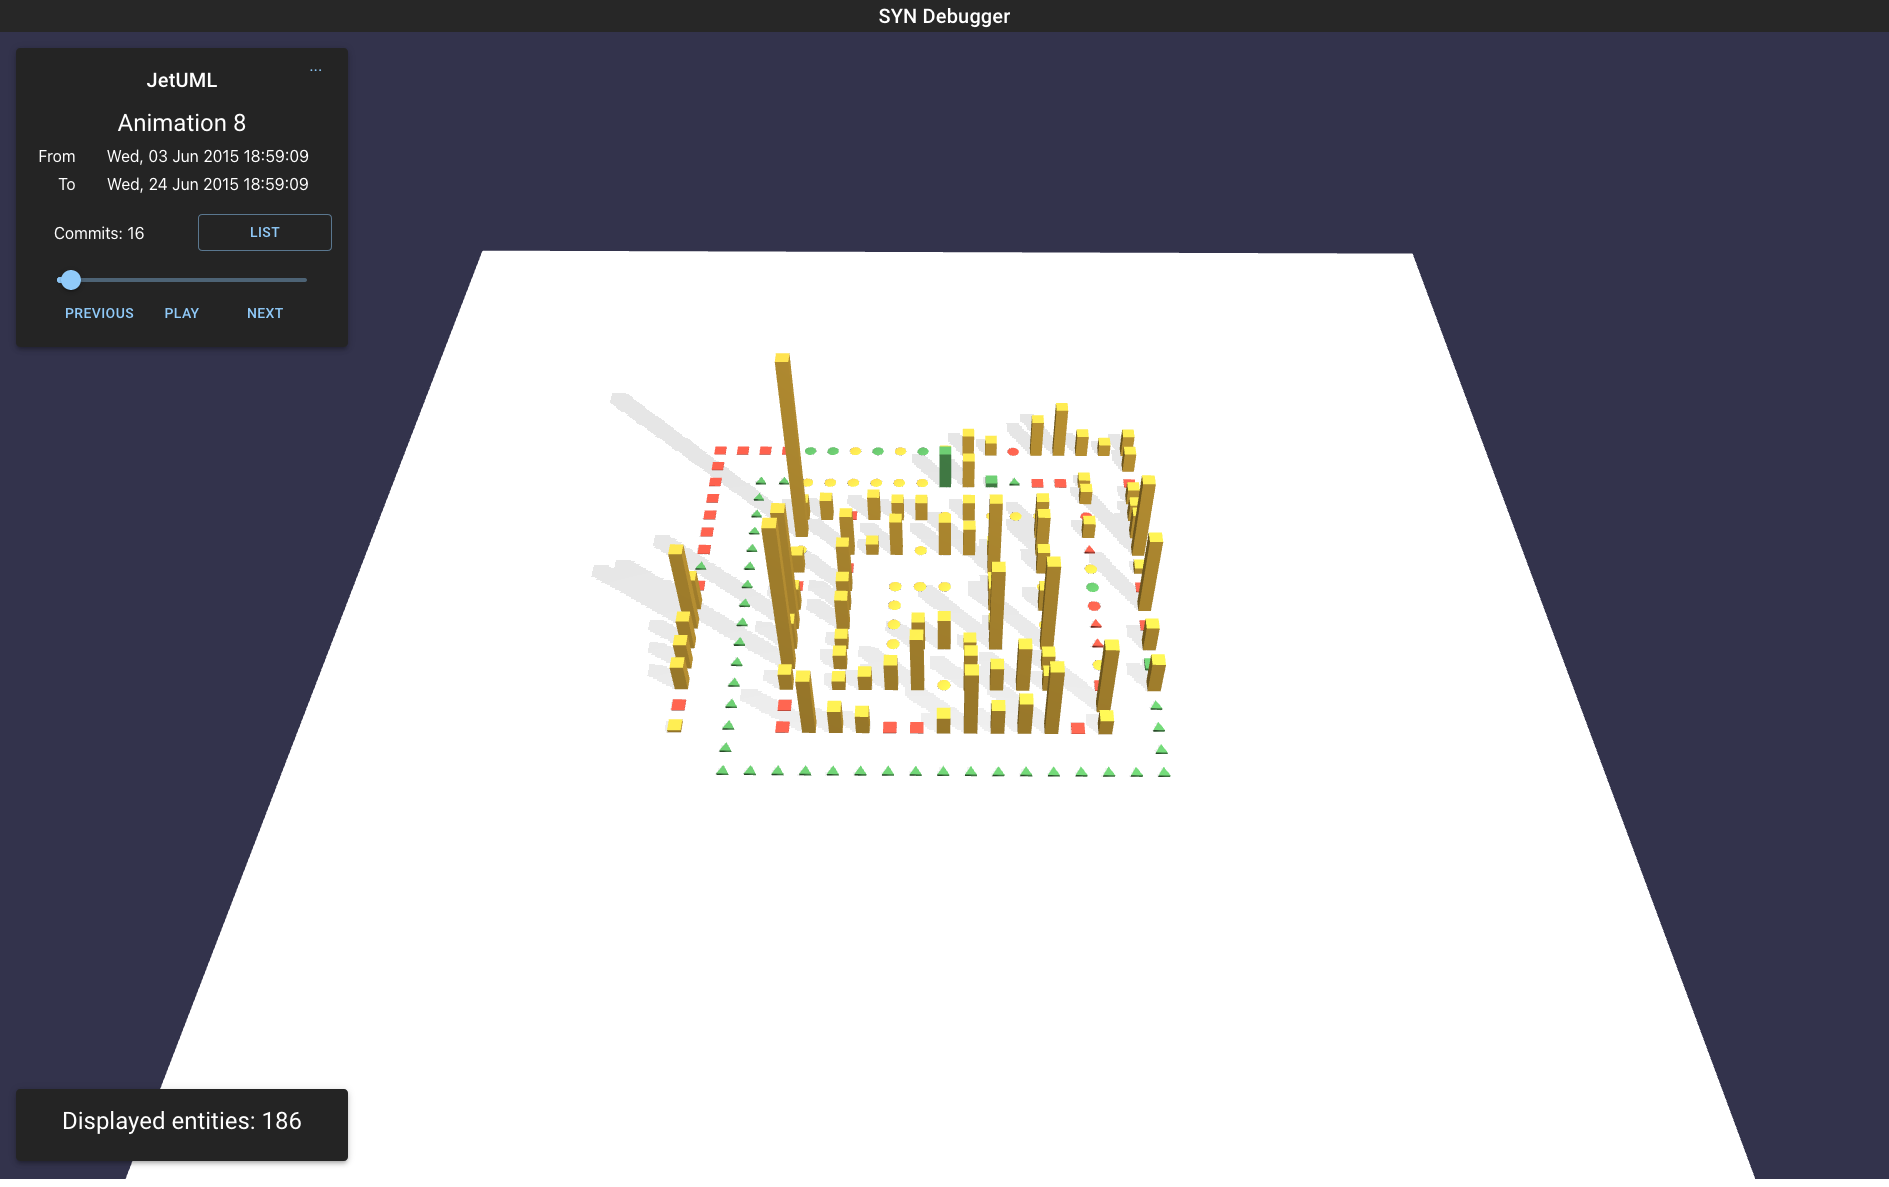
\includegraphics[width=\textwidth]{SYNUI-deletedshadow.png}
    \caption{Visualization of JetUML with shadows, deleted entities and custom shapes for non-java files.}
    \label{fig:deletedshadow}
\end{figure}


The Visual Inspector is a helpful tool for understanding and debugging SYN's analysis process. However, it has performance issues in rendering large systems. The main problem stems browser environment as it has limited resources. Even though Javascript has APIs to support a high-performance rendering of 3D graphics,\footnote{\url{https://developer.mozilla.org/en-US/docs/Web/API/WebGL_API}} we experienced a significant frame rate (frames per second, FPS) drop when rendering large systems. To overcome this limitation and prove the versatility of our approach, we rendered large systems with POV-Ray,\footnote{\url{http://www.povray.org}} an open-source tool for creating high-quality three-dimensional graphics. It works with \texttt{pov} files containing instructions to specify how the image should be rendered. We developed an extension of SYN that, given a View, produces a \texttt{pov} file for each AnimationFrame, following the same approach adopted in the Visual Inspector. \autoref{fig:povteaser} provides an example of a big system rendered with POV-Ray.

\begin{figure}
    \center
    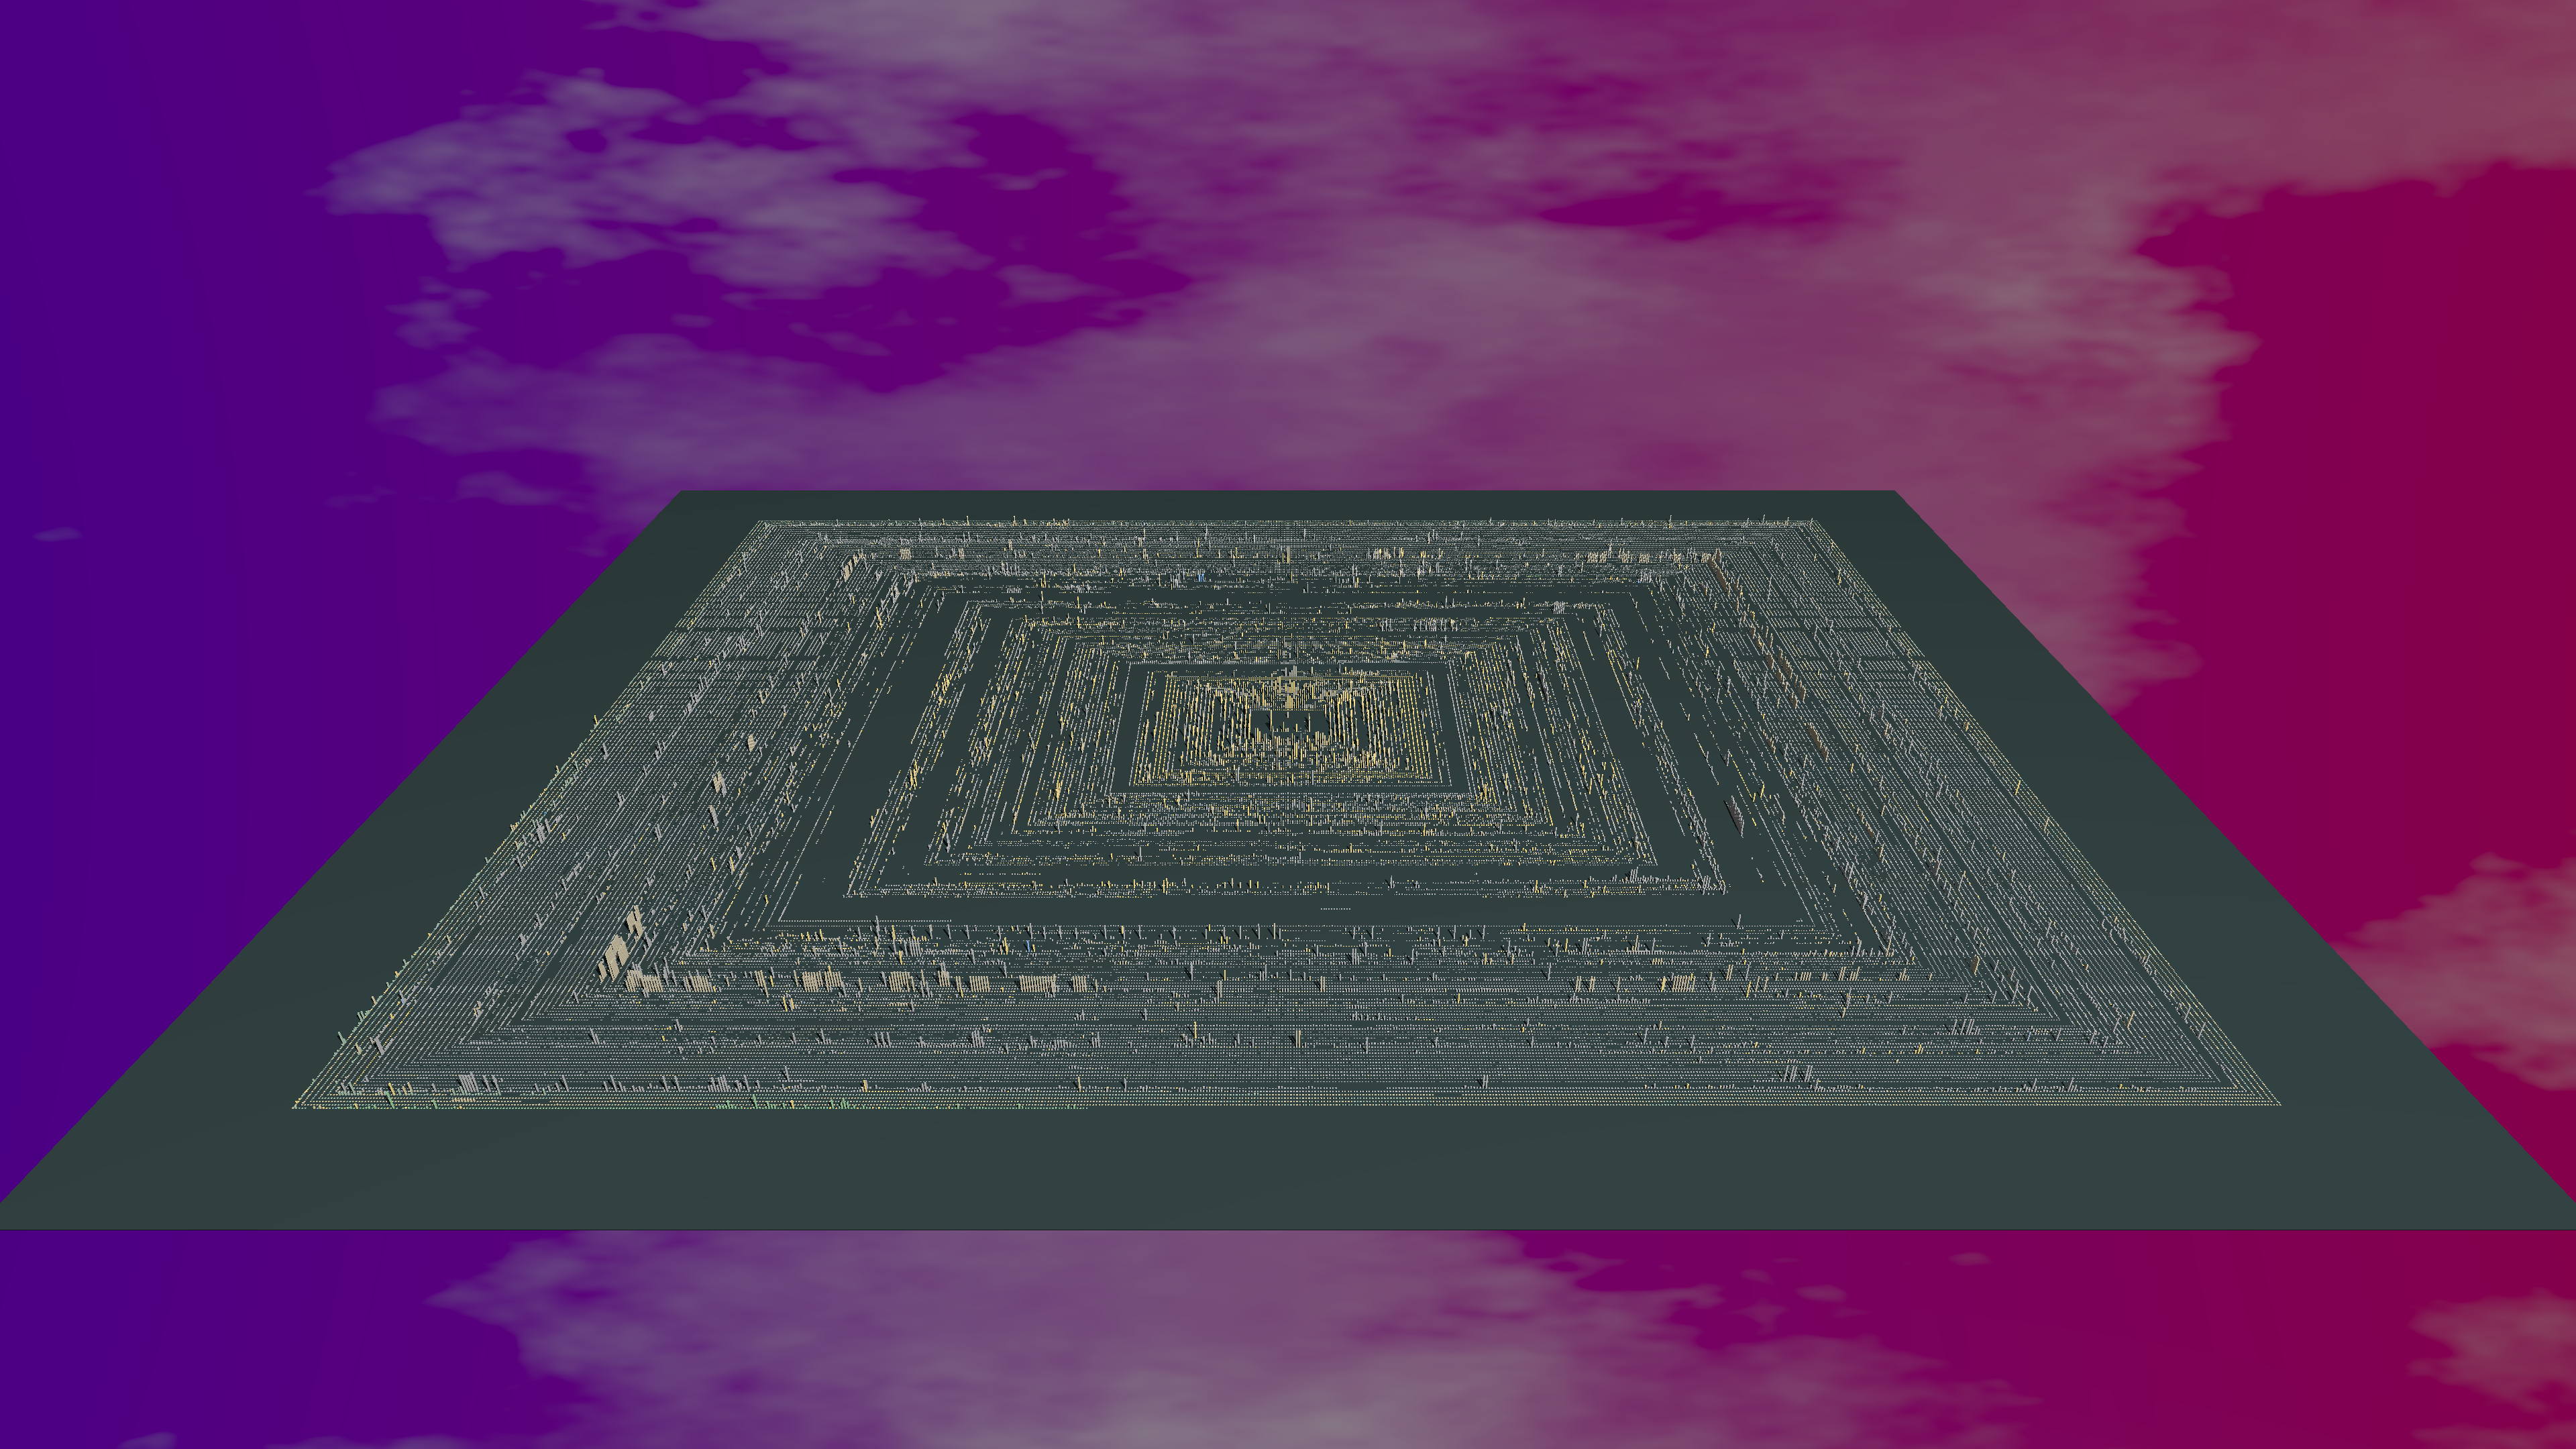
\includegraphics[width=\textwidth]{LibreOfficeTeaser.png}
    \caption{Example of a system rendered with POV-Ray}
    \label{fig:povteaser}
\end{figure}

\section{Audio}
SYN implements the auralization approach (see \autoref{sec:audioApproach}) in the Core component. 
Its implementation uses Sonic Pi\footnote{\url{https://sonic-pi.net}} to compose melodies. Sonic Pi is a code-based creation tool written in Ruby. It enables you to write and modify code live to make music. To do that, it defines a domain-specific language to compose melodies procedurally. For example, the instruction \texttt{play 60} plays the 60th note on the piano (selected by default). 

\begin{figure}
    \center
    \includegraphics[width=\textwidth]{SonicPi.png}
    \caption{Interface of SonicPi}
    \label{fig:sonicpi}
\end{figure}

This implementation aims to produce a depiction of the evolution to support the 3D visualization. To do that, we built our auditive approach on the ViewAnimation. Therefore, we extract from each frame the following metrics: number of files added, number of files removed, and number of commits. The idea is to use their value to generate three tracks, each depending upon a metric. We play each AnimationFrame for one second. We employed the following sounds:
\begin{itemize}
    \item Bass drums: to represent the number of commits in an AnimationFrame. We decided to normalize the values retrieved by this metric in the interval $\left[60,200\right]$. Consequently, when the animation with less commit in the evolution is displayed, the retrieved by this metric is 60, and the same goes for the maximum. We used this value to set the BPM of this track. The amplitude is always at 1 (the maximum). Under those circumstances, users can understand how active the period represented by the played AnimationFrame was by paying attention to the number of bass drums heard each second.
    \item Bass sound: to represent the number of deleted files in an AnimationFrame. We use the number of deleted files to determine the repetition and the amplitude of the sound. The value is normalized to $\left[1,4\right]$ for the repetition and $\left[0.1,0.8\right]$ for the amplitude.
    \item Electric sound: to represent the number of files added in an AnimationFrame.  We use the number of added files to determine the repetition and the amplitude of the sound. The value is normalized to $\left[1,8\right]$ for the repetition and $\left[0.2,0.85\right]$ for the amplitude.
\end{itemize}

\autoref{app:SonicPiLinux} shows the code we developed to implement this mapping. 
%In the first three lines, there are three arrays containing the metric's values. Before being used, these values are normalized by the \texttt{rescale} function. 

To debug our auralization approach, we developed a Python application that queries the server and controls SonicPi. The application works as follows: first, it queries the GraphQL server to retrieve the view of a project. Once the view is returned, it extracts from each AnimationFrame the needed metric values. Then these values are sent to SonicPi through a protocol called Open Sound Protocol (OSC). Finally, it renders one graph for each metric to let us associate each metric value with a sound. To do that, we used a black dot representing the current AnimationFrame. 

\autoref{fig:Bokeh} shows the interface of the debugger. Each chart represents a metric, and the black dot (synchronized with SonicPi) represents the AnimationFrame being auralized. 


\begin{figure}
    \center
    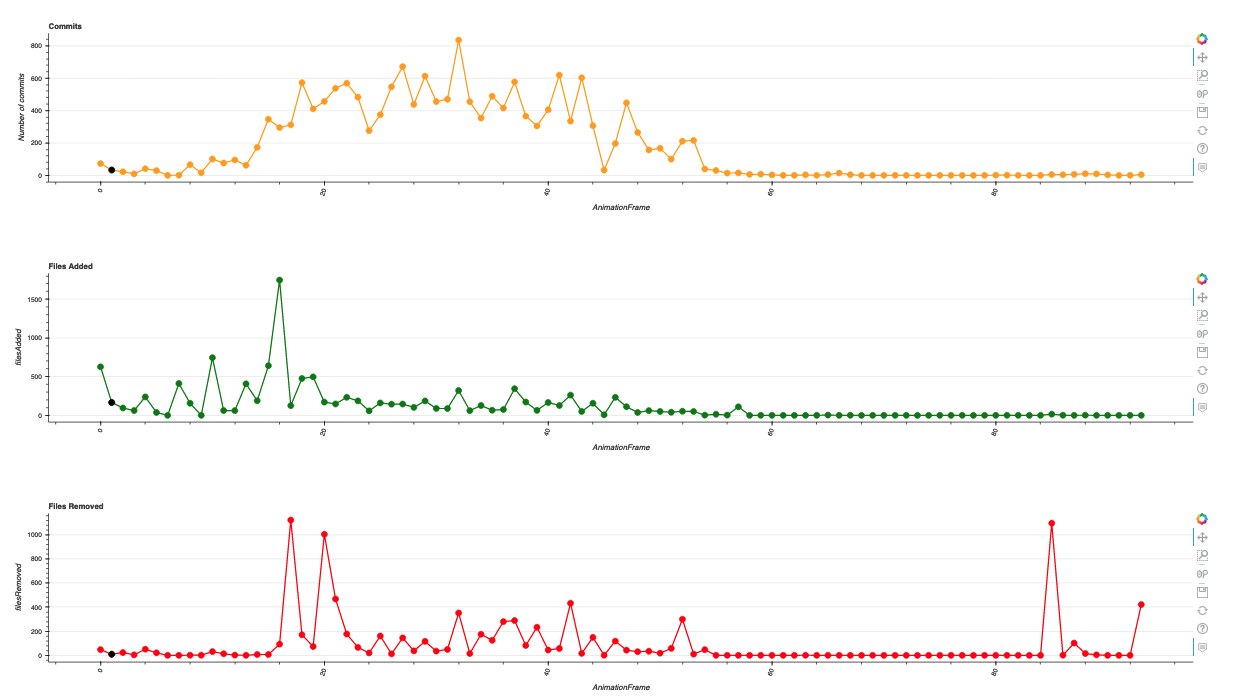
\includegraphics[width=\textwidth]{Bokeh.png}
    \caption{Charts used to debug the melody}
    \label{fig:Bokeh}
\end{figure}

